\appendix
\section{Architectural details}
\label{sec:appendix_architecture}
\mypar{Network backbone.} 
Table~\ref{tab:backbone} illustrates the details of our \emph{backbone} architecture ($f_{\theta}$ in the main paper).
For both variants, we use a ResNet-50~\cite{he2016deep} until the final convolutional layer of the 4-th stage.
In order to obtain a higher spatial resolution in deep layers, we reduce the output stride to 8 by using convolutions with stride 1. 
Moreover, we increase the receptive field by using dilated convolutions~\cite{chen2018deeplab}.
Specifically, we set the stride to 1 and the dilation rate to 2 in the $3{\times}3$ conv layer of \texttt{conv4\_1}. 
Differently to the original ResNet-50, there is no downsampling in \texttt{conv4\_x}.
We also add to the backbone an \emph{adjust} layer (a $1{\times}1$ convolutional layer with 256 output channels). 
Examplar and search patches share the network's parameters from \texttt{conv1} to \texttt{conv4\_x}, while the parameters of the \textit{adjust} layer are not shared.
The output features of the adjust layer are then depth-wise cross-correlated, resulting a feature map of size 17{$\times$}17.

\mypar{Network heads.} 
The network architecture of the branches of both variants are shows in Table~\ref{tab:three} and~\ref{tab:two}.
The \texttt{conv5} block in both variants contains a normalisation layer and ReLU non-linearity while \texttt{conv6} only consists of a $1{\times}1$ convolutional layer.

\mypar{Mask refinement module.} 
With the aim of producing a more accurate object mask, we follow the strategy of~\cite{SharpMask}, which merges low and high resolution features using multiple~\textit{refinement} modules made of upsampling layers and skip connections.
Figure~\ref{fig:u} gives an example of refinement module $U_3$, while Figure~\ref{fig:rm} illustrates how a mask is generated with stacked refinement modules.



\newcommand{\blocka}[2]{\multirow{3}{*}{\(\left[\begin{array}{c}\text{3$\times$3, #1}\\[-.1em] \text{3$\times$3, #1} \end{array}\right]\)$\times$#2}
}
\newcommand{\blockb}[3]{\multirow{3}{*}{\(\left[\begin{array}{c}\text{1$\times$1, #2}\\[-.1em] \text{3$\times$3, #2}\\[-.1em] \text{1$\times$1, #1}\end{array}\right]\)$\times$#3}
}
\renewcommand\arraystretch{1.1}
\setlength{\tabcolsep}{2pt}
\begin{table}[h]
\begin{center}
\resizebox{1\linewidth}{!}{
\begin{tabular}{c|c|c|c}
\hline
\textit{block} & \textit{examplar} output size  & \textit{search} output size & \textit{backbone} \\
\hline
conv1 & 61$\times$61 & 125$\times$125 & 7$\times$7, 64, stride 2\\
\hline
\multirow{4}{*}{conv2\_x} &\multirow{4}{*}{31$\times$31} & \multirow{4}{*}{63$\times$63} & 3$\times$3 max pool, stride 2 \\
  &  &  &\blockb{256}{64}{3} \\
  &  &  \\
  &  &  \\
\hline
\multirow{3}{*}{conv3\_x} &\multirow{3}{*}{15$\times$15}  &\multirow{3}{*}{31$\times$31}  & \blockb{512}{128}{4} \\
  &  &  \\
  &  &  \\
\hline
\multirow{3}{*}{conv4\_x} &\multirow{3}{*}{15$\times$15} &\multirow{3}{*}{31$\times$31}   & \blockb{1024}{256}{6} \\
  &  &   \\
  &  &   \\
\hline
		\textit{adjust} & $15{\times}15$ & $31{\times}31$ & $1{\times}1$, 256\\
\hline
xcorr&   \multicolumn{2}{c|}{17 $\times$ 17} & depth-wise \\
\hline
\end{tabular}
}
\end{center}
\caption{Backbone architecture. Details of each building block are shown in square brackets.
}
\label{tab:backbone}
\vspace{-0.2cm}
\end{table}



\renewcommand\arraystretch{1.1}
\setlength{\tabcolsep}{2pt}
\begin{table}
\begin{center}
\resizebox{0.75\linewidth}{!}{
\begin{tabular}{c|c|c|c}
\hline
\textit{block}  & score   & box  & mask\\
\hline
conv5& 1 $\times$ 1, 256  &  1 $\times$ 1, 256  & 1 $\times$ 1, 256  \\

\hline
conv6 & 1 $ \times $ 1, 2$k$ & 1 $\times$ 1, 4$k$  & 1 $\times$ 1, (63 $ \times $ 63) \\

\hline
\end{tabular}
}
\end{center}
\caption{Architectural details of the \textit{three-branch} head.
$k$ denotes the number of anchor boxes per RoW.
}
\label{tab:three}
\vspace{-0.2cm}
\end{table}





\renewcommand\arraystretch{1.1}
\setlength{\tabcolsep}{2pt}
\begin{table}
\begin{center}
\resizebox{0.6\linewidth}{!}{
\begin{tabular}{c|c|c}
\hline
\textit{block} & score  & mask\\
\hline
conv5& 1 $\times$ 1, 256  &  1 $\times$ 1, 256    \\

\hline
conv6 & 1 $ \times $ 1, 1 & 1 $\times$ 1, (63 $ \times $ 63) \\

\hline
\end{tabular}
}
\end{center}
\caption{Architectural details of the \textit{two-branch} head.
}
\label{tab:two}
\vspace{-0.2cm}
\end{table}


\begin{figure}
\begin{center}
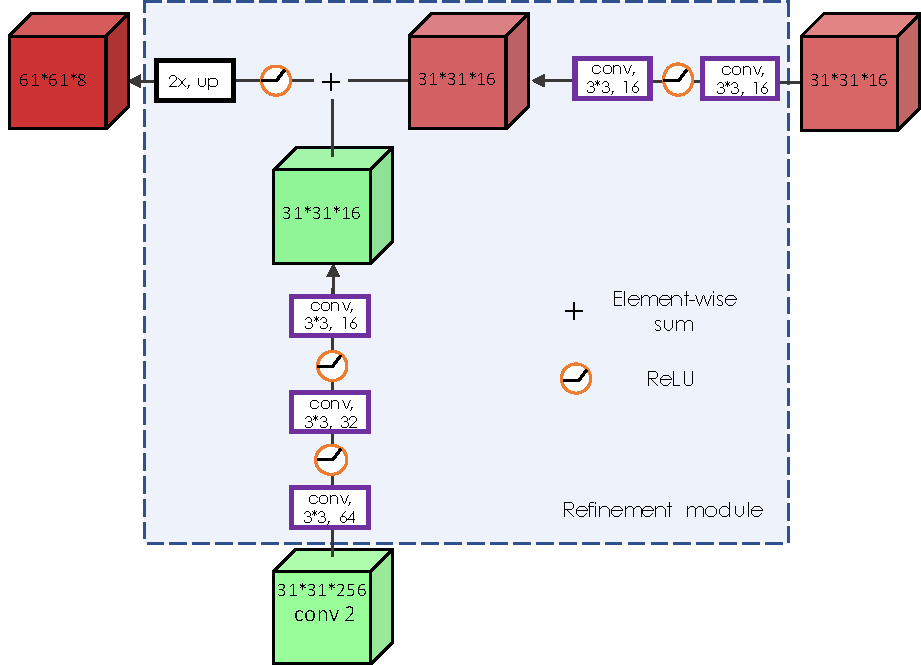
\includegraphics[width=0.4\textwidth]{img/u.pdf}
\end{center}
\vspace{-0.2cm}
\caption{Example of a refinement module $U_3$.}
\label{fig:u}
\end{figure}

\section{Further qualitative results}
\label{sec:appendix_qualitative}
\begin{figure}
\begin{center}
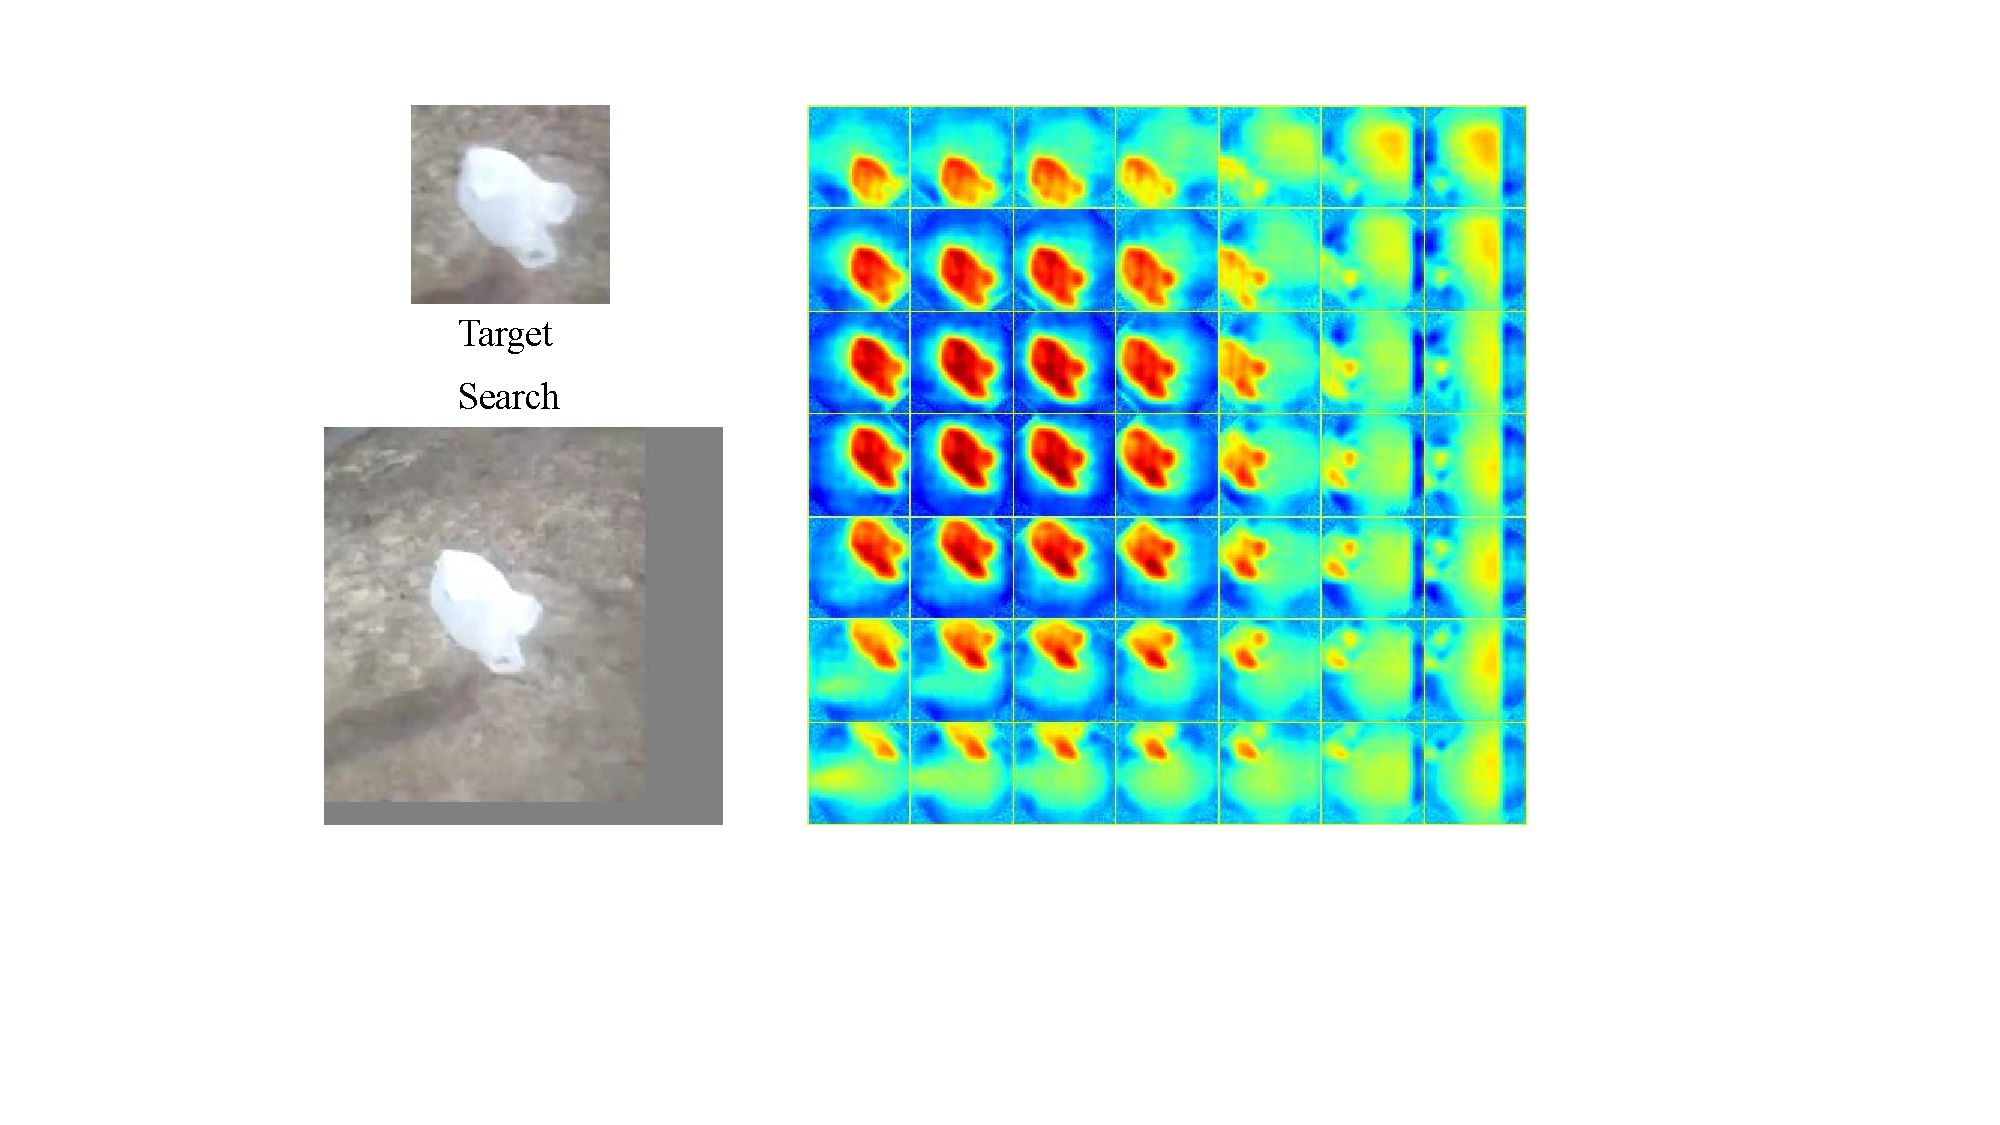
\includegraphics[width=0.47 \textwidth]{supp/heatmap_loc.pdf}
\end{center}
\vspace{-0.2cm}
\caption{Score maps from the mask branch at different locations.}
\label{fig:map}
\end{figure}

\mypar{Different masks at different locations.}
Our model generates a mask for each RoW.
During inference, we rely on the score branch to select the final output mask (using the location attaining the maximum score).
The example of Figure~\ref{fig:map} illustrates the multiple output masks produced by the mask branch, each corresponding to a different RoW.

\mypar{Benchmark sequences.}
More qualitative results for VOT and DAVIS sequences are shown in Figure~\ref{fig:appendix_vot18} and~\ref{fig:appendix_davis16}.

\begin{figure*}[h]
\begin{center}
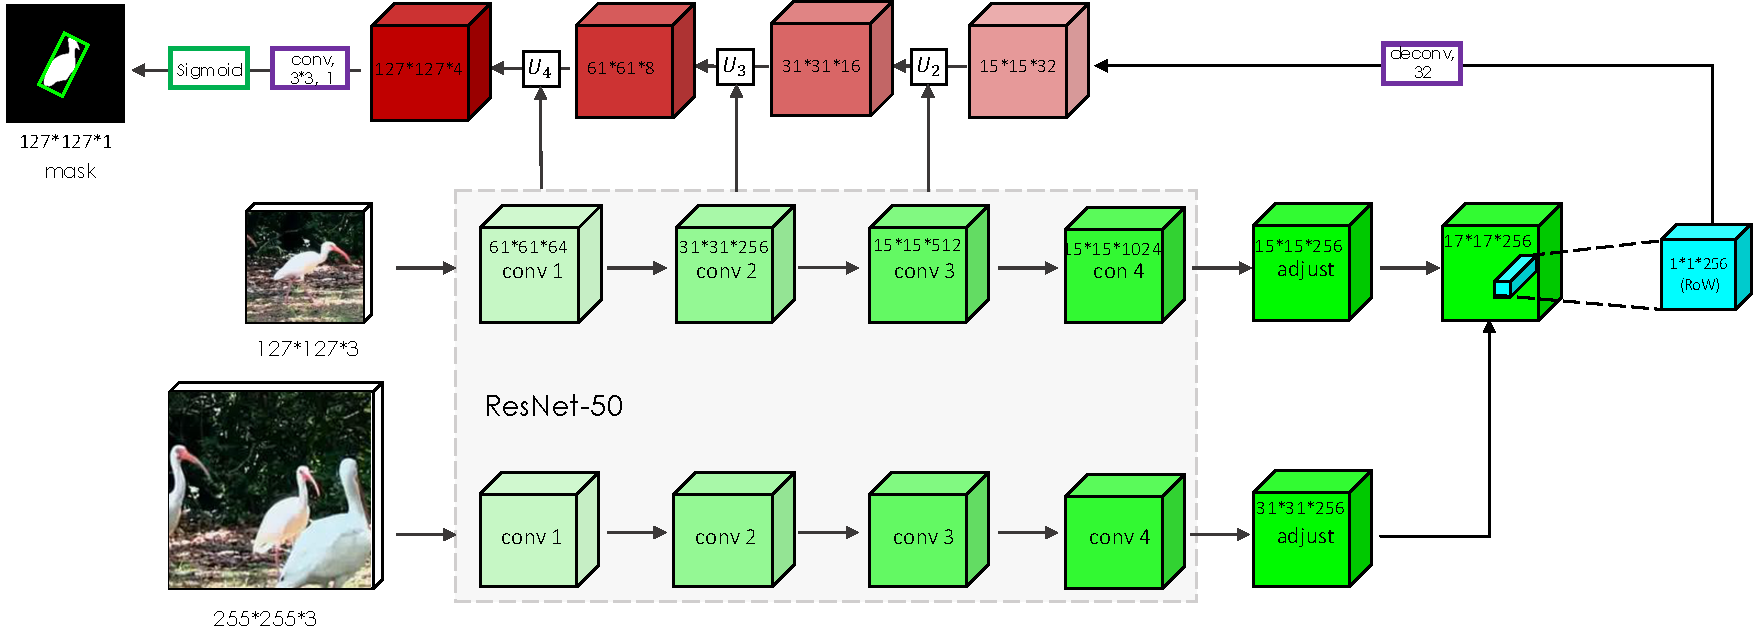
\includegraphics[width=0.9 \textwidth]{img/rm.pdf}
\end{center}
\vspace{-0.2cm}
\caption{Schematic illustration of the stacked refinement modules.}
\label{fig:rm}
\end{figure*}

\begin{figure*}
\centering
\setlength{\tabcolsep}{0.25ex}

\begin{tabular}
{cccccc cccccc}
\mbox{\centering\rotatebox[x=-0.55cm]{90}{\small{butterfly}}}
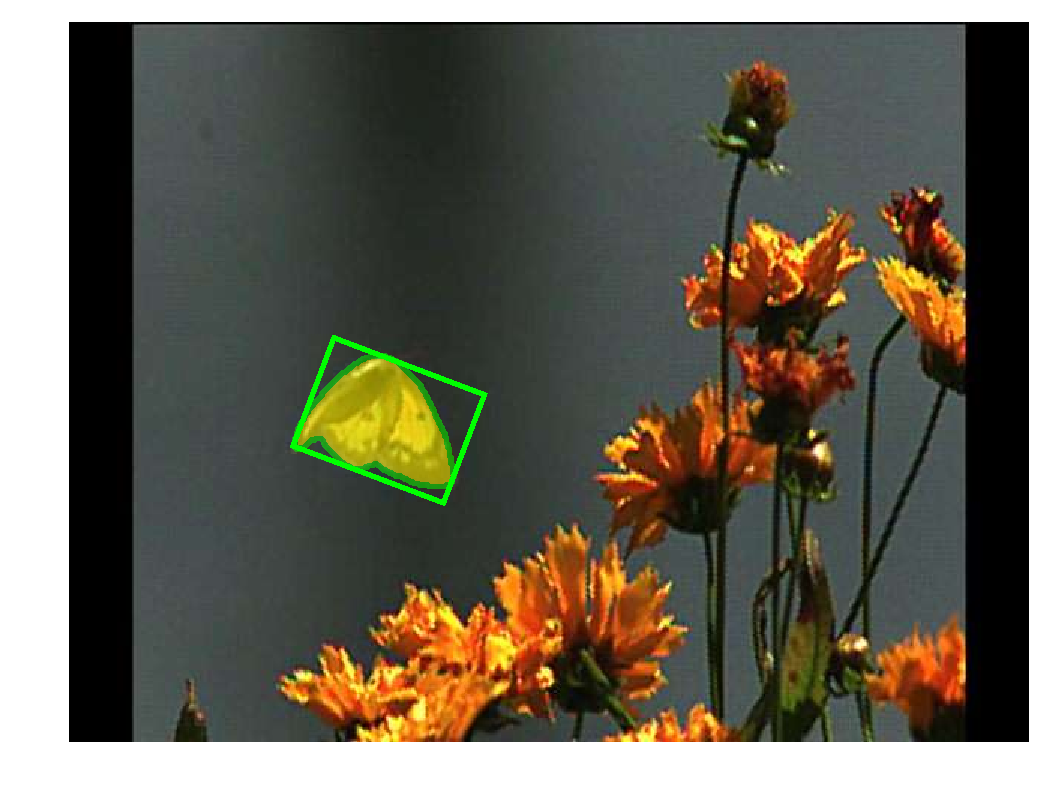
\includegraphics[trim={2.5cm 2cm 2.5cm 0.5cm},clip,width = 1.1in]{supp/vot2018/pdf/butterfly/00020}
&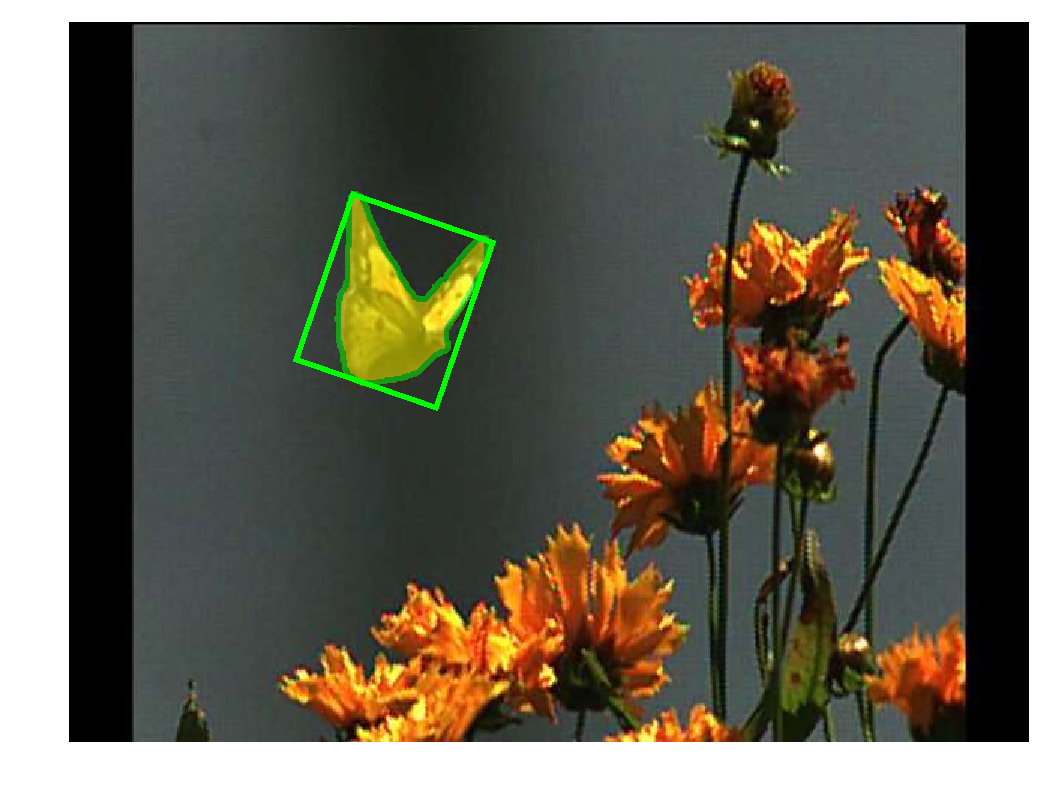
\includegraphics[trim={2.5cm 2cm 2.5cm 0.5cm},clip,width = 1.1in]{supp/vot2018/pdf/butterfly/00034}
& 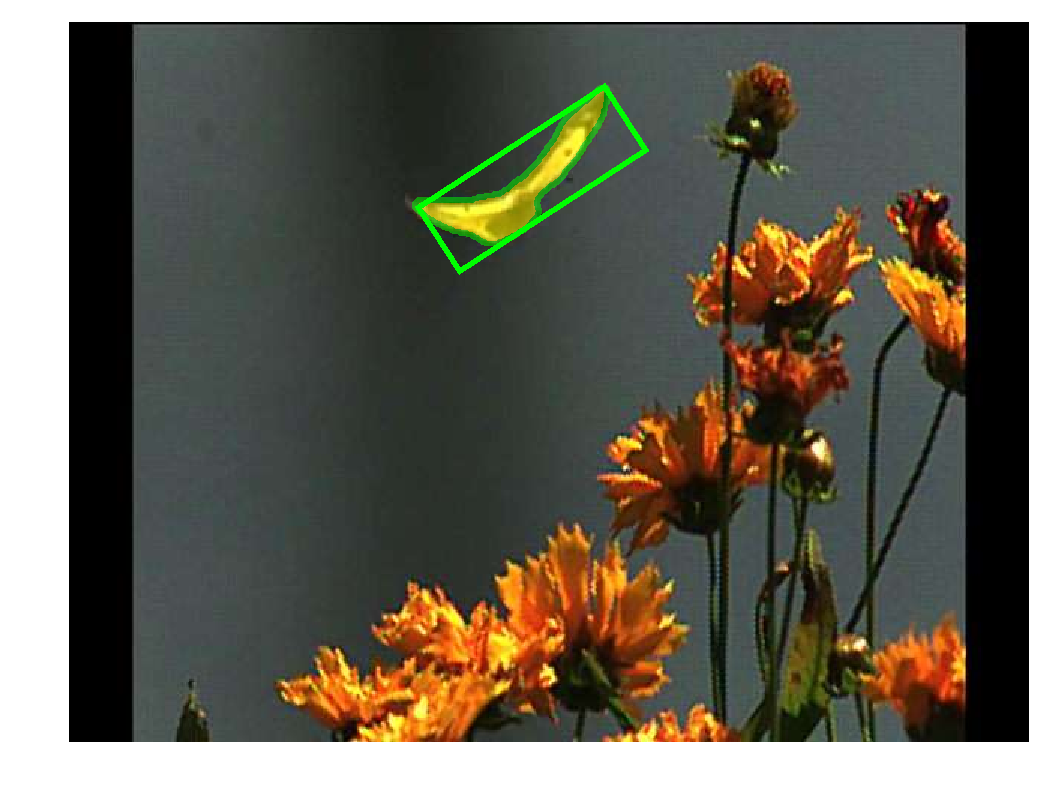
\includegraphics[trim={2.5cm 2cm 2.5cm 0.5cm},clip,width = 1.1in]{supp/vot2018/pdf/butterfly/00052}
& 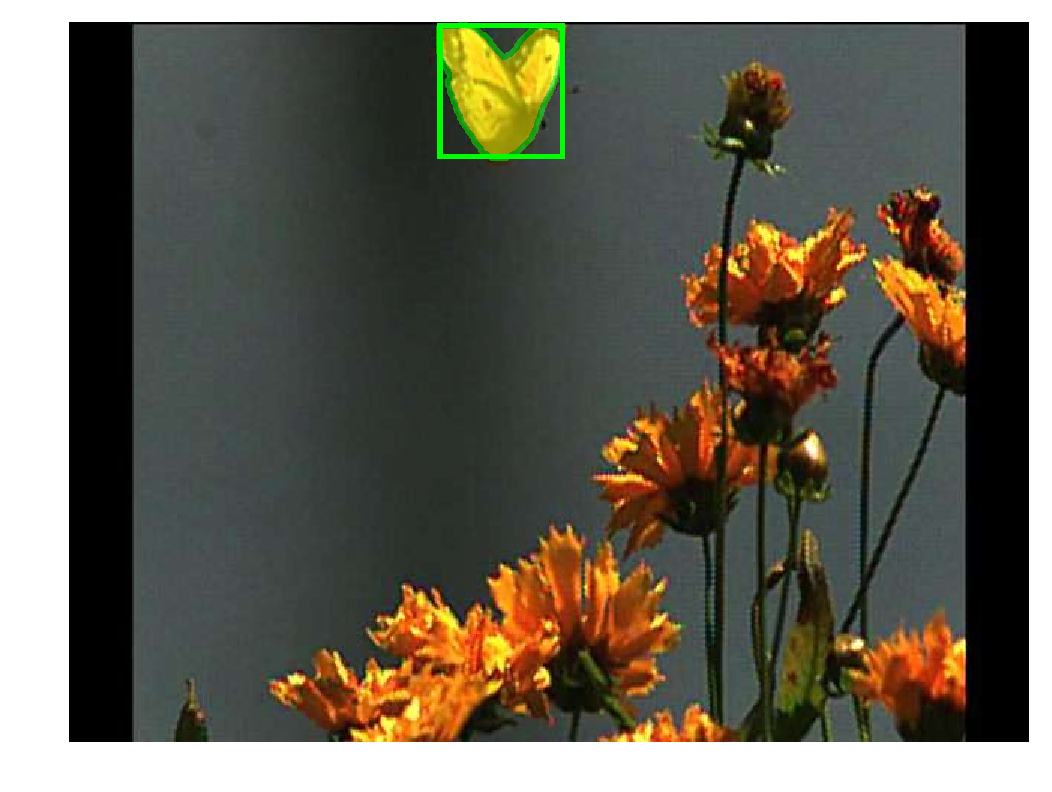
\includegraphics[trim={2.5cm 2cm 2.5cm 0.5cm},clip,width = 1.1in]{supp/vot2018/pdf/butterfly/00077}
& 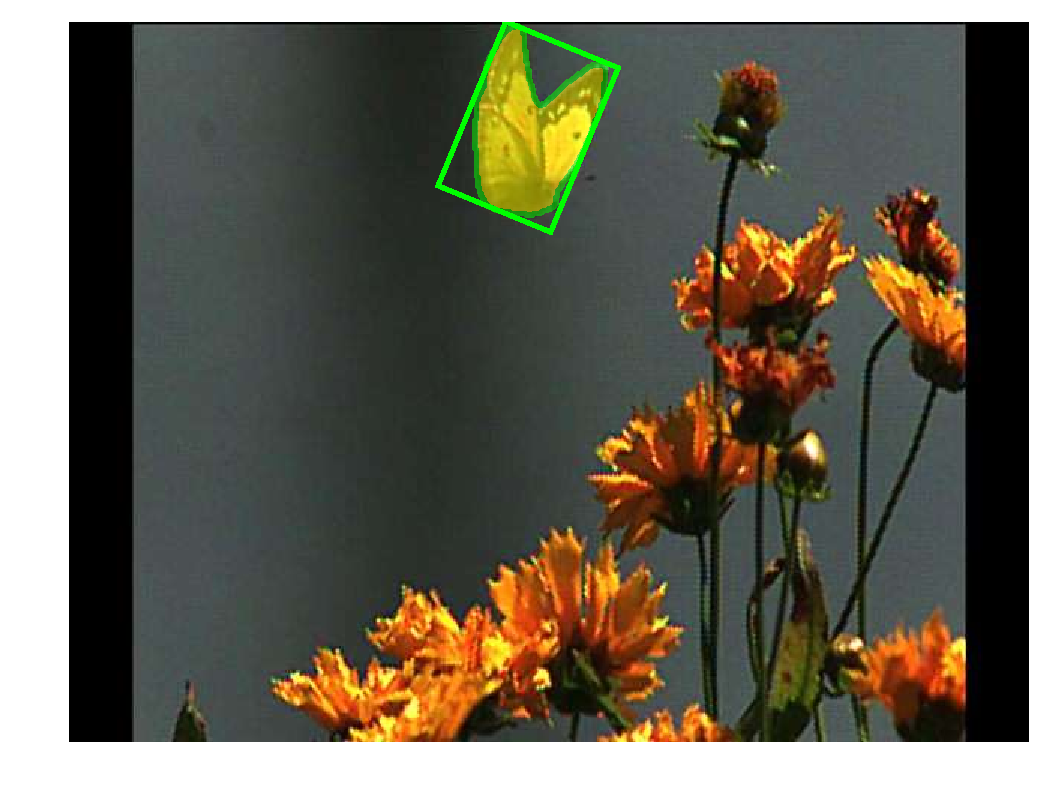
\includegraphics[trim={2.5cm 2cm 2.5cm 0.5cm},clip,width = 1.1in]{supp/vot2018/pdf/butterfly/00123}
& 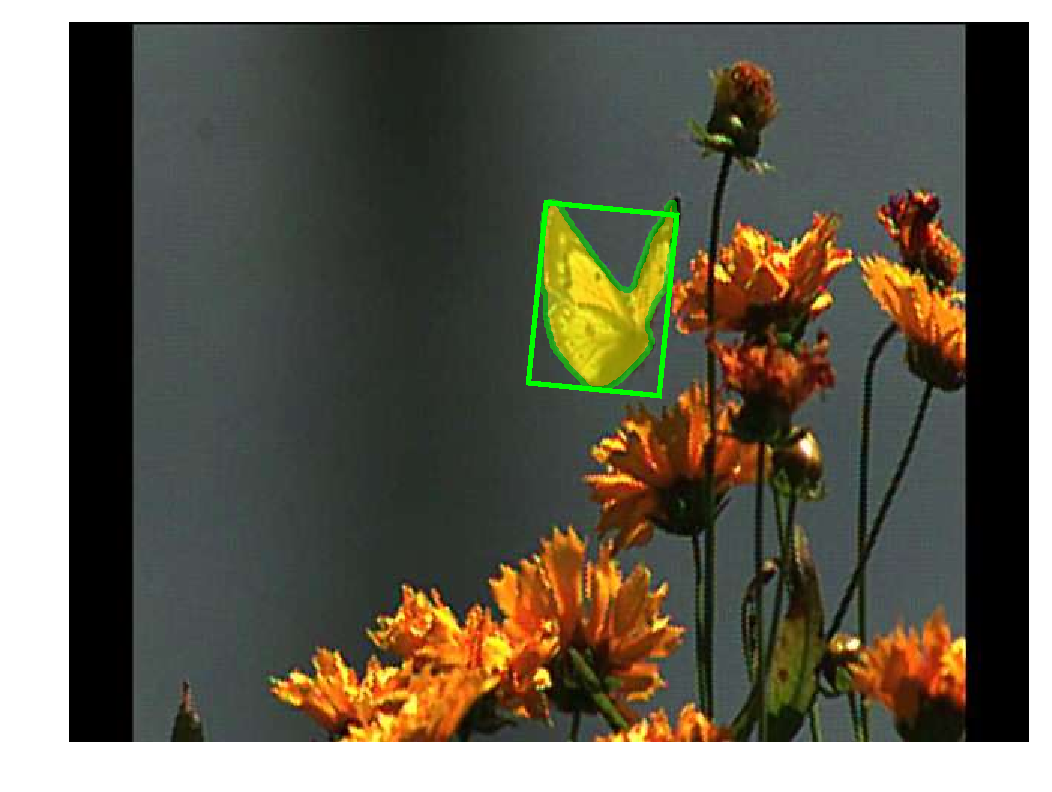
\includegraphics[trim={2.5cm 2cm 2.5cm 0.5cm},clip,width = 1.1in]{supp/vot2018/pdf/butterfly/00145}
\\
\mbox{\rotatebox[x=-0.55cm]{90}{\small{crabs1}}}
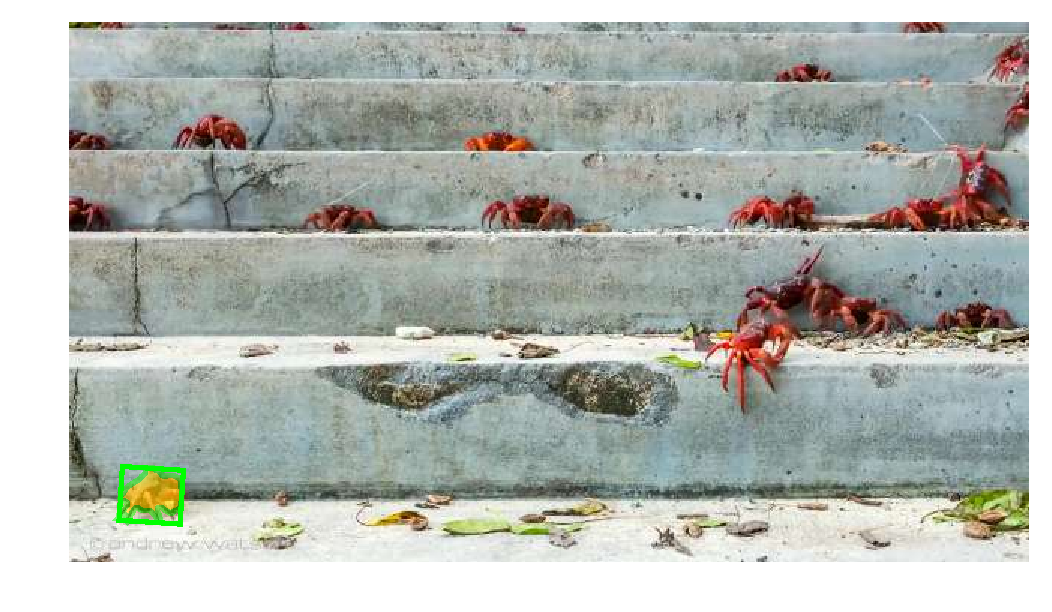
\includegraphics[trim={2.5cm 1cm 2.5cm 1cm},clip,width = 1.1in]{supp/vot2018/pdf/crabs1/00002}
&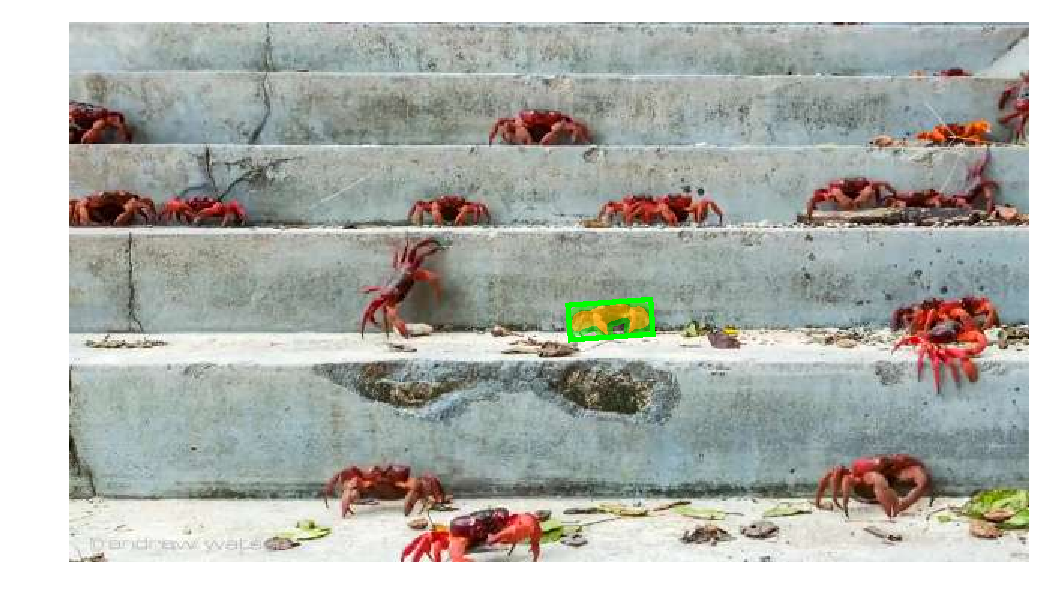
\includegraphics[trim={2.5cm 1cm 2.5cm 1cm},clip,width = 1.1in]{supp/vot2018/pdf/crabs1/00045}
& 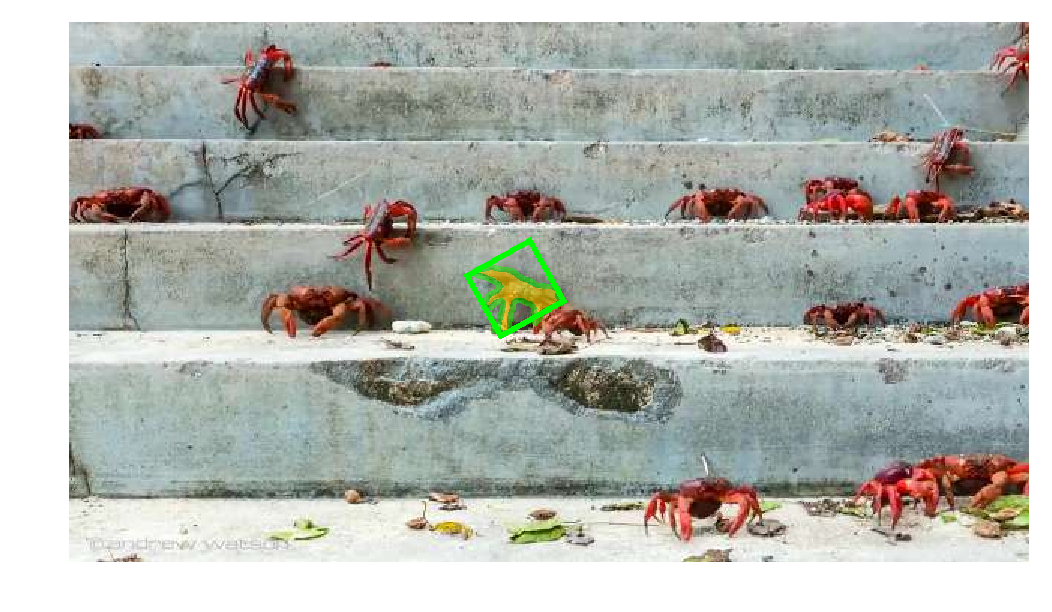
\includegraphics[trim={2.5cm 1cm 2.5cm 1cm},clip,width = 1.1in]{supp/vot2018/pdf/crabs1/00079}
& 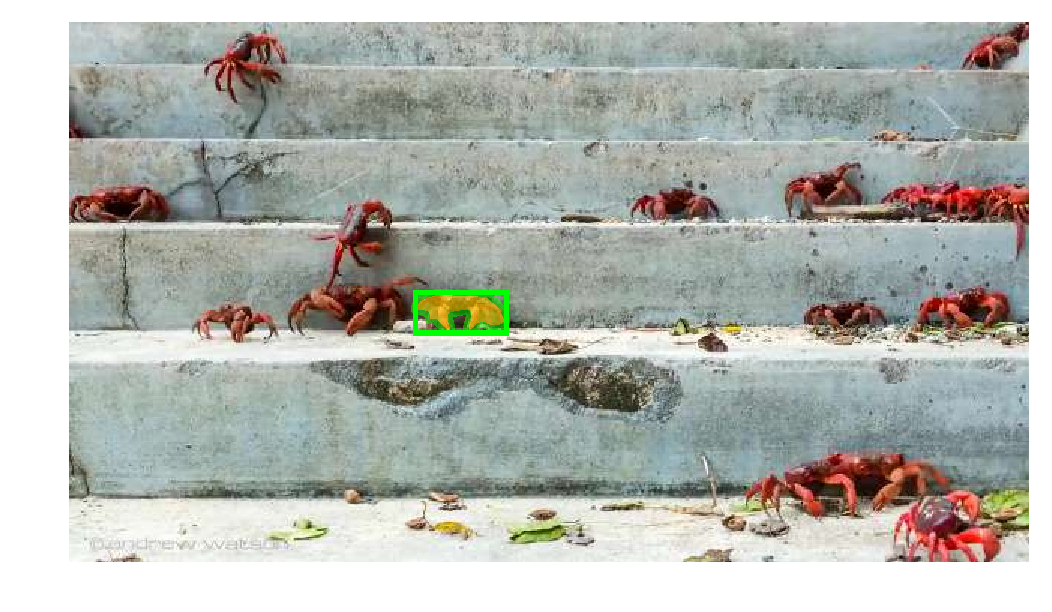
\includegraphics[trim={2.5cm 1cm 2.5cm 1cm},clip,width = 1.1in]{supp/vot2018/pdf/crabs1/00087}
& 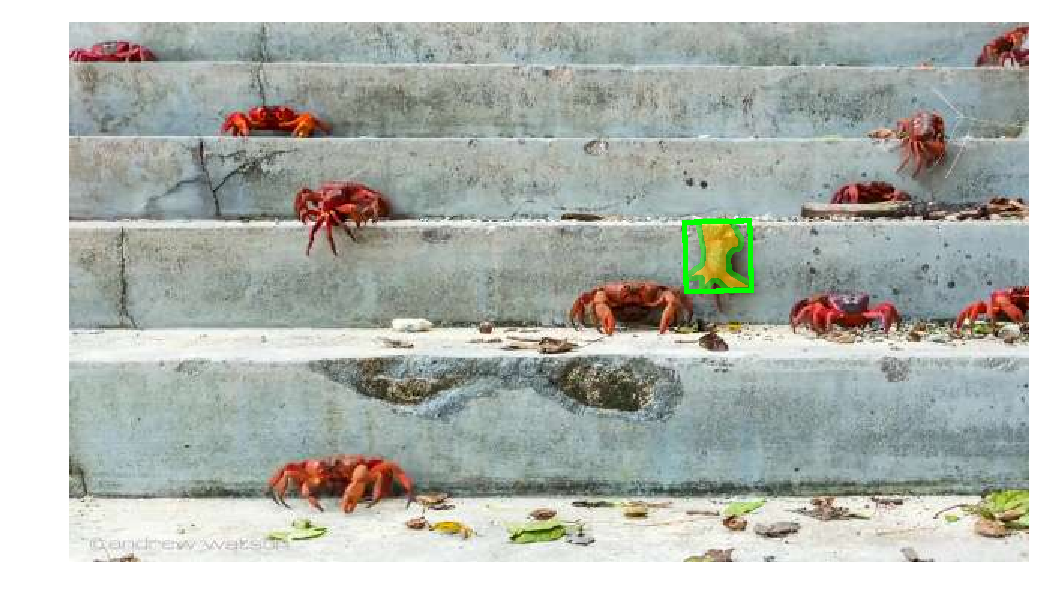
\includegraphics[trim={2.5cm 1cm 2.5cm 1cm},clip,width = 1.1in]{supp/vot2018/pdf/crabs1/00104}
& 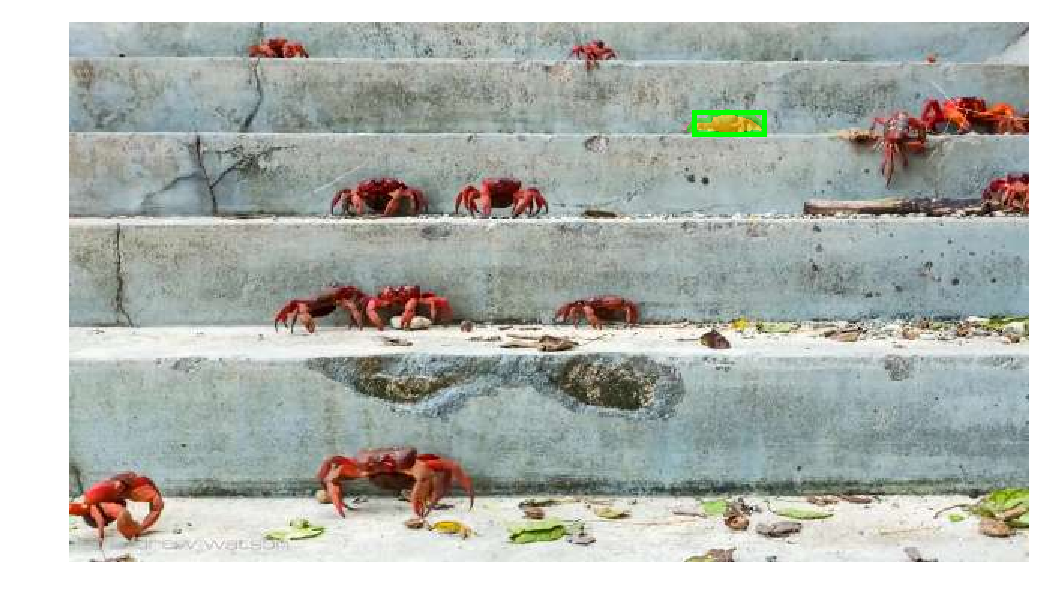
\includegraphics[trim={2.5cm 1cm 2.5cm 1cm},clip,width = 1.1in]{supp/vot2018/pdf/crabs1/00134}
\\
\mbox{\rotatebox[x=-0.0cm]{90}{\small{iceskater1}}}
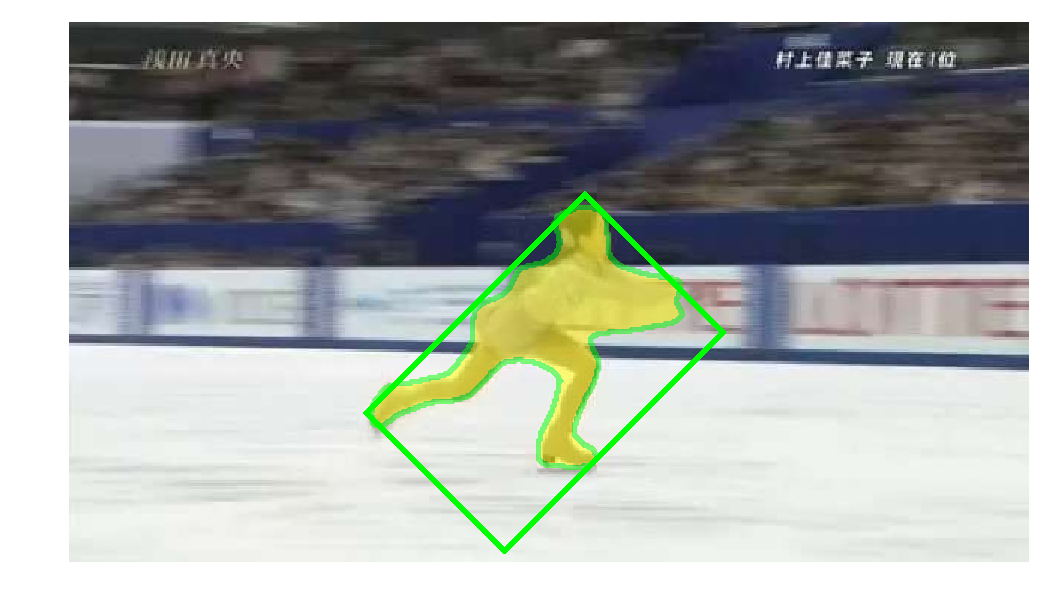
\includegraphics[trim={2.5cm 1cm 2.5cm 1cm},clip,width = 1.1in]{supp/vot2018/pdf/iceskater1/00102}
&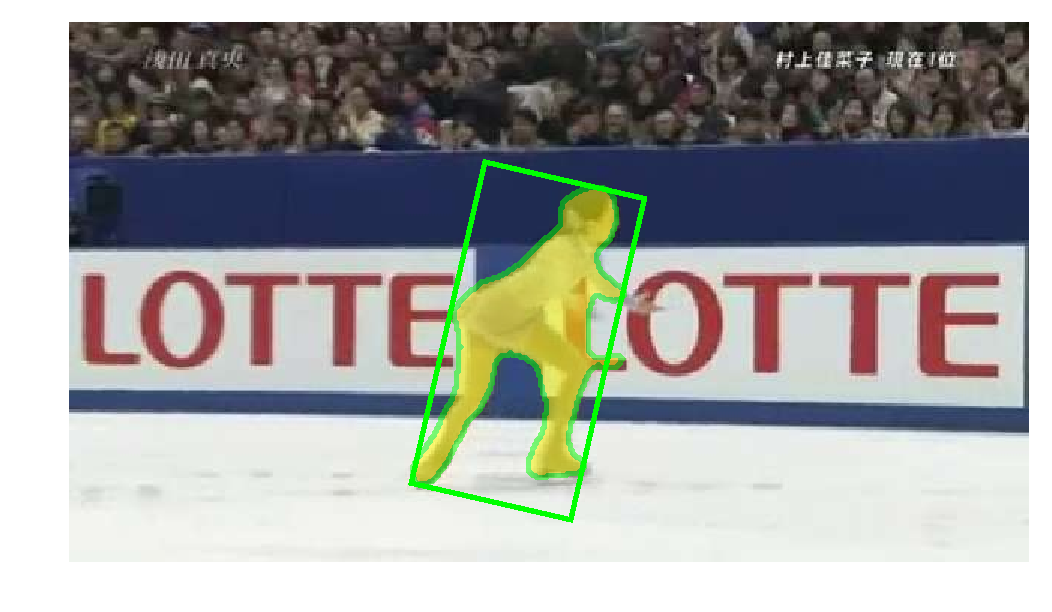
\includegraphics[trim={2.5cm 1cm 2.5cm 1cm},clip,width = 1.1in]{supp/vot2018/pdf/iceskater1/00203}
& 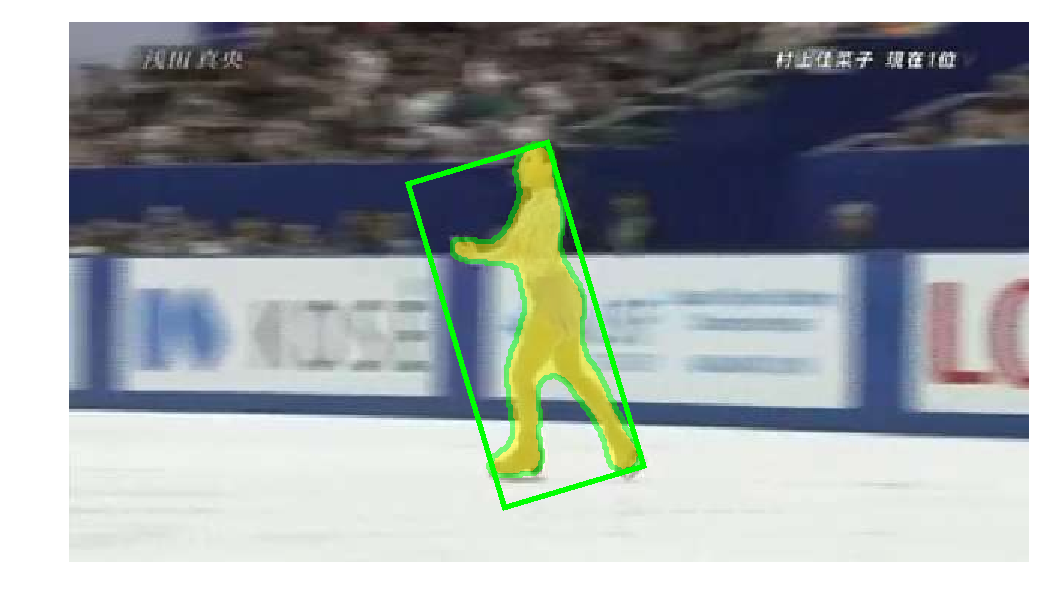
\includegraphics[trim={2.5cm 1cm 2.5cm 1cm},clip,width = 1.1in]{supp/vot2018/pdf/iceskater1/00301}
& 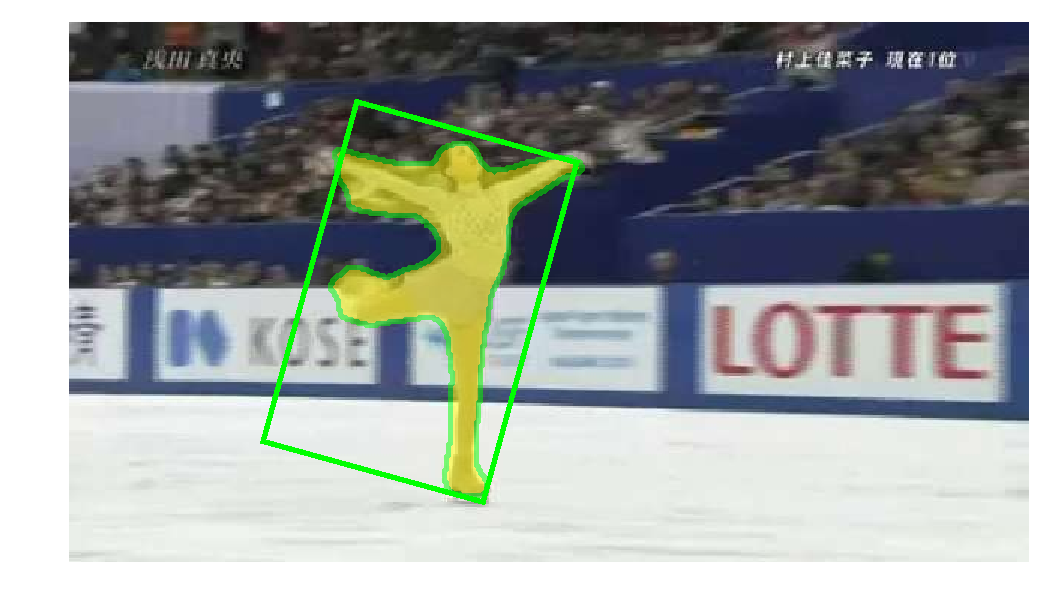
\includegraphics[trim={2.5cm 1cm 2.5cm 1cm},clip,width = 1.1in]{supp/vot2018/pdf/iceskater1/00402}
& 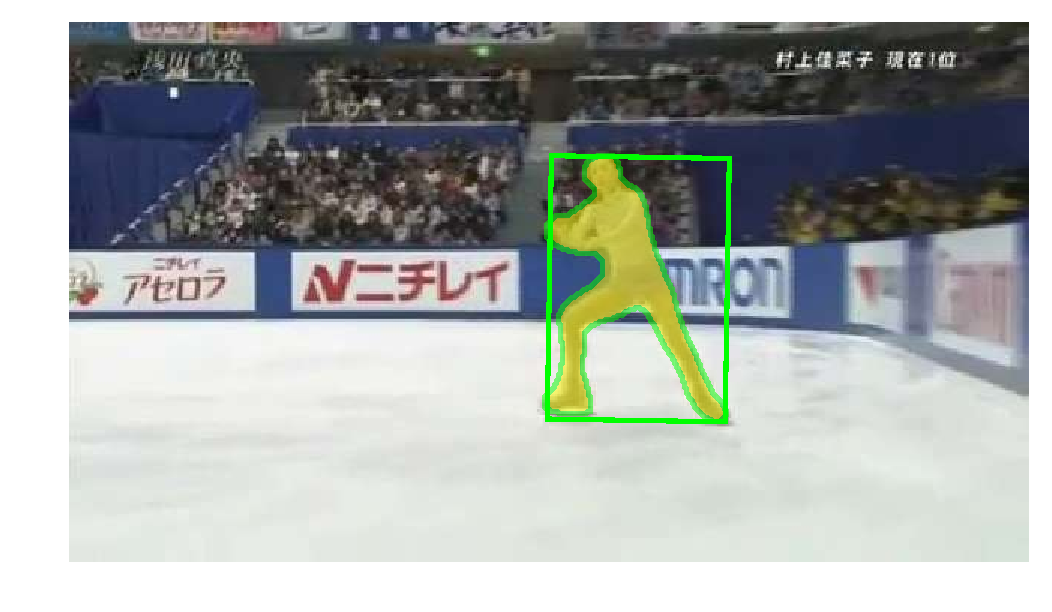
\includegraphics[trim={2.5cm 1cm 2.5cm 1cm},clip,width = 1.1in]{supp/vot2018/pdf/iceskater1/00540}
& 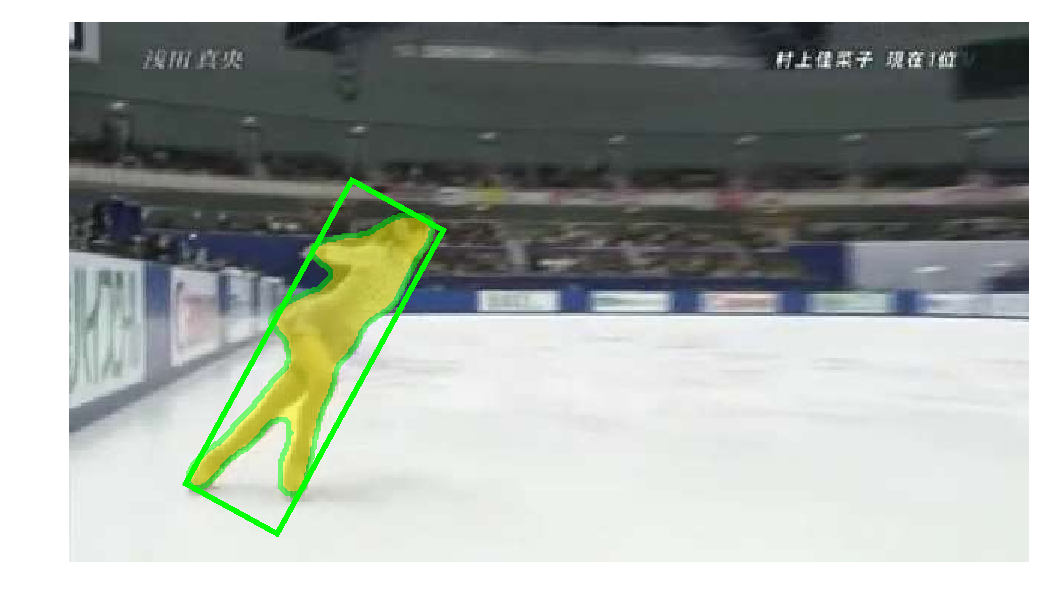
\includegraphics[trim={2.5cm 1cm 2.5cm 1cm},clip,width = 1.1in]{supp/vot2018/pdf/iceskater1/00609}
\\
\mbox{\rotatebox[x=-0.15cm]{90}{\small{iceskater2}}}
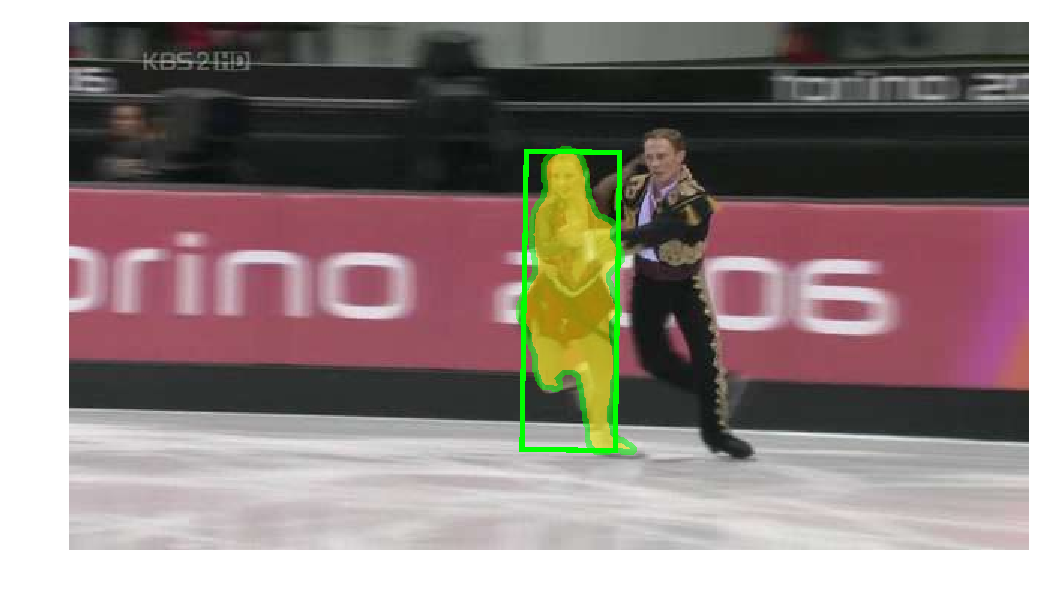
\includegraphics[trim={2.5cm 1cm 2.5cm 1cm},clip,width = 1.1in]{supp/vot2018/pdf/iceskater2/00086}
&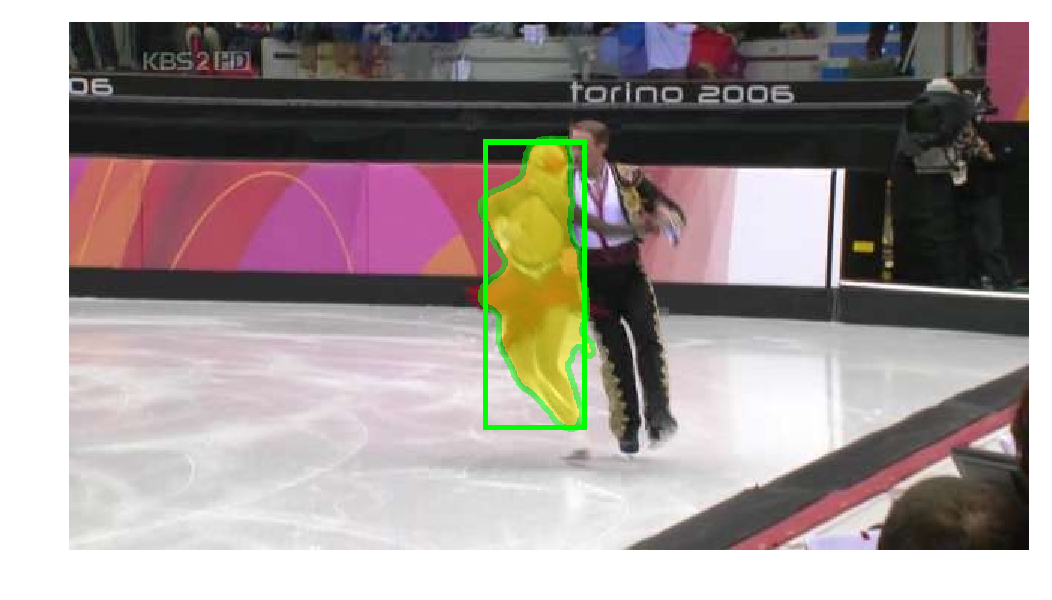
\includegraphics[trim={2.5cm 1cm 2.5cm 1cm},clip,width = 1.1in]{supp/vot2018/pdf/iceskater2/00193}
& 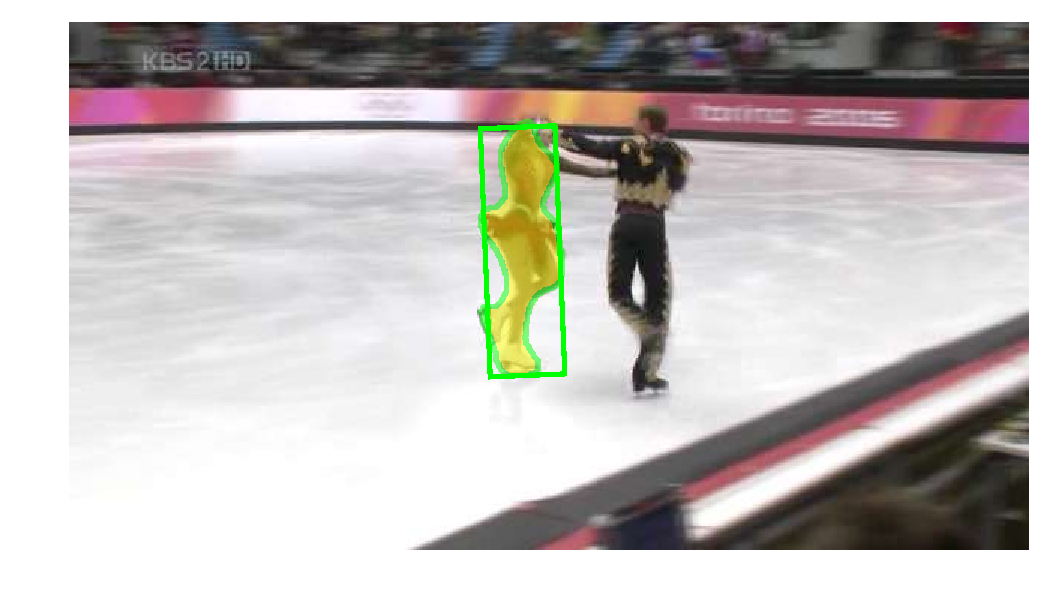
\includegraphics[trim={2.5cm 1cm 2.5cm 1cm},clip,width = 1.1in]{supp/vot2018/pdf/iceskater2/00320}
& 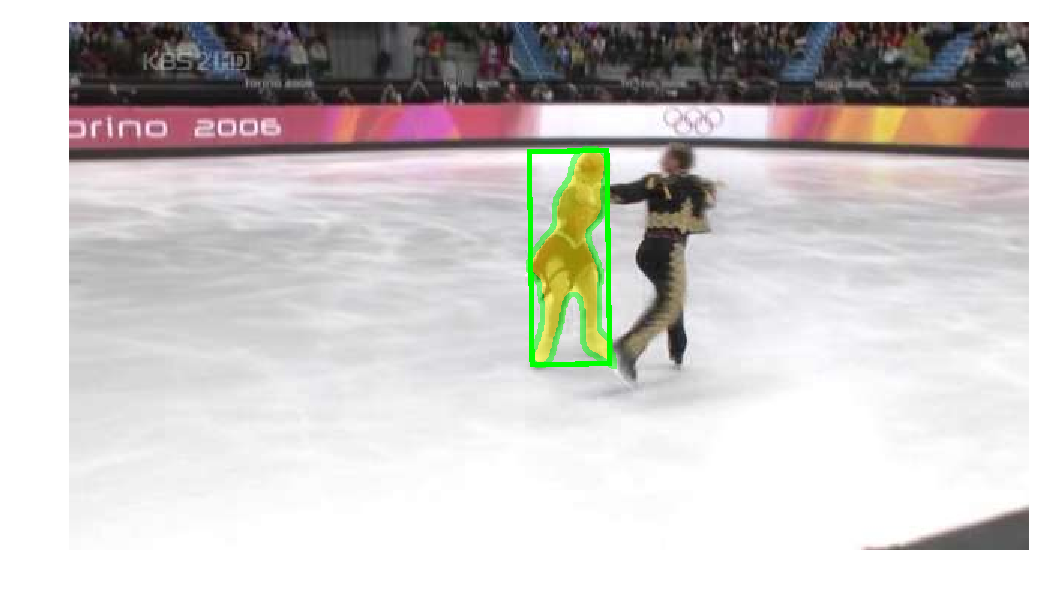
\includegraphics[trim={2.5cm 1cm 2.5cm 1cm},clip,width = 1.1in]{supp/vot2018/pdf/iceskater2/00347}
& 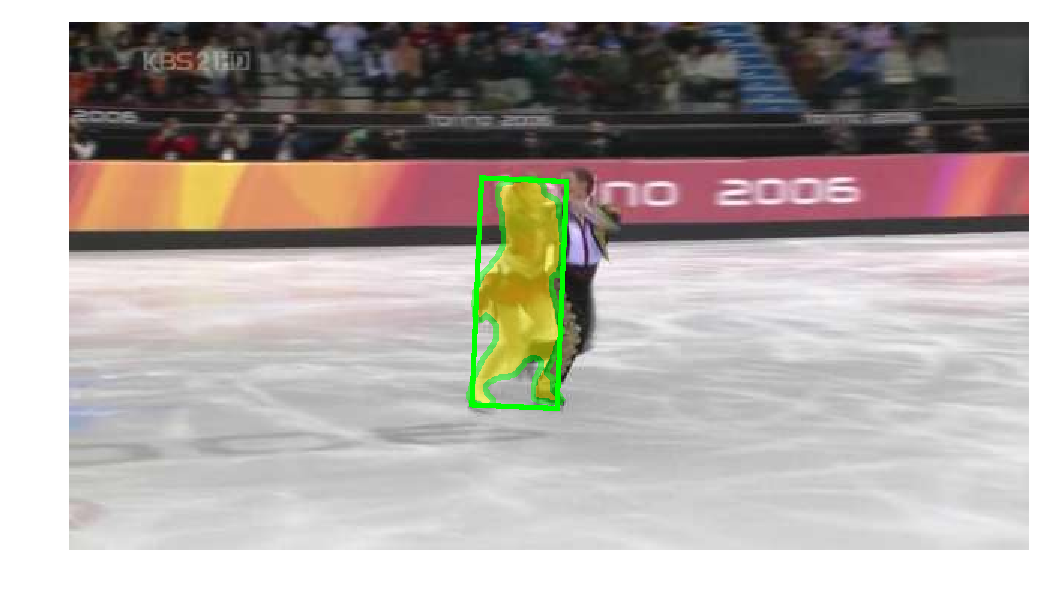
\includegraphics[trim={2.5cm 1cm 2.5cm 1cm},clip,width = 1.1in]{supp/vot2018/pdf/iceskater2/00437}
& 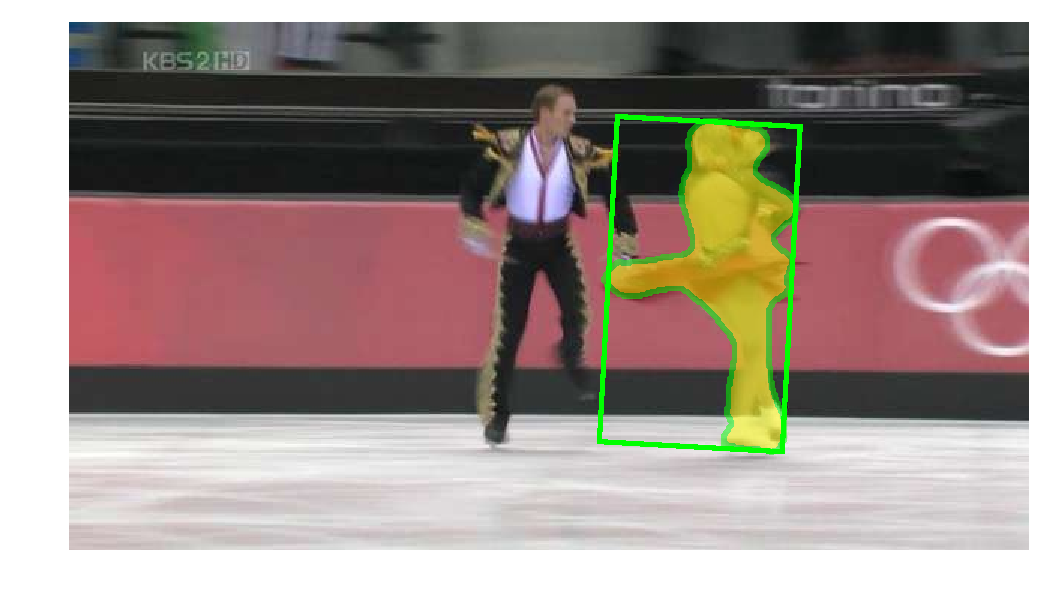
\includegraphics[trim={2.5cm 1cm 2.5cm 1cm},clip,width = 1.1in]{supp/vot2018/pdf/iceskater2/00607}
\\
\mbox{\rotatebox[x=-0.1cm]{90}{\small{motocross1}}}
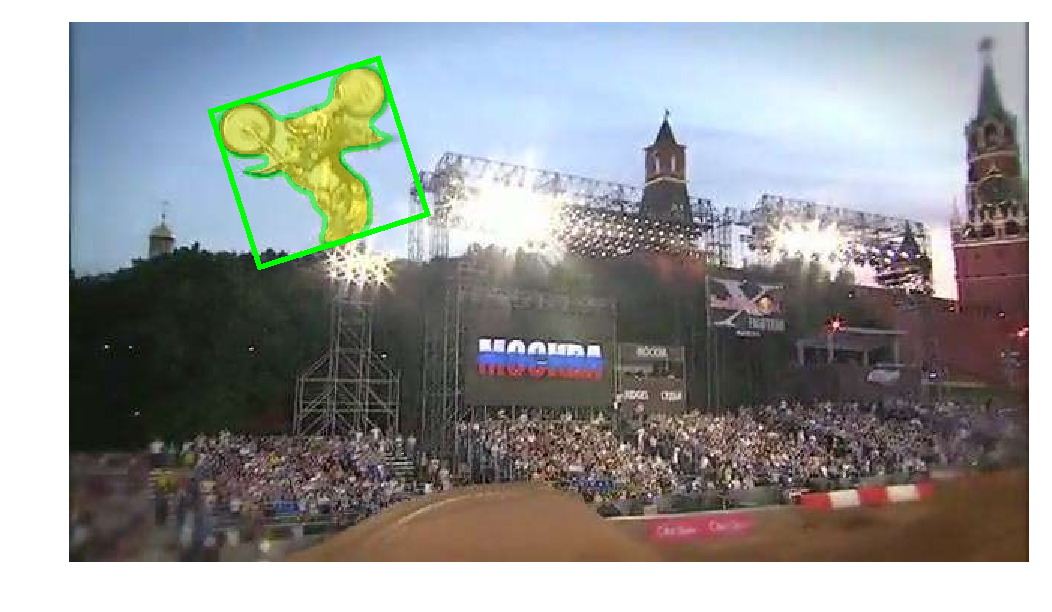
\includegraphics[trim={2.5cm 1cm 2.5cm 1cm},clip,width = 1.1in]{supp/vot2018/pdf/motocross1/00005}
&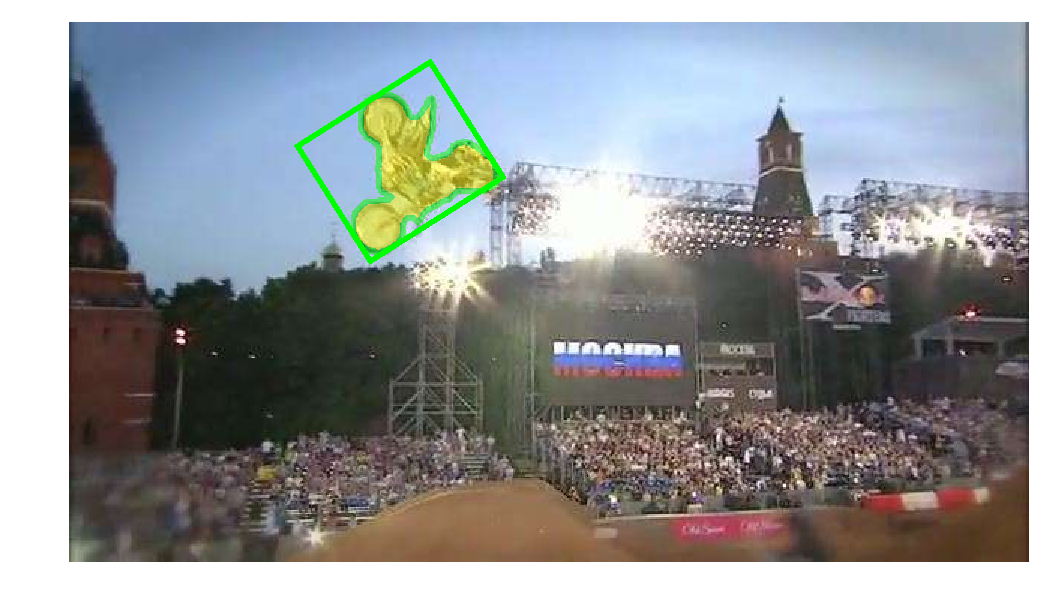
\includegraphics[trim={2.5cm 1cm 2.5cm 1cm},clip,width = 1.1in]{supp/vot2018/pdf/motocross1/00018}
& 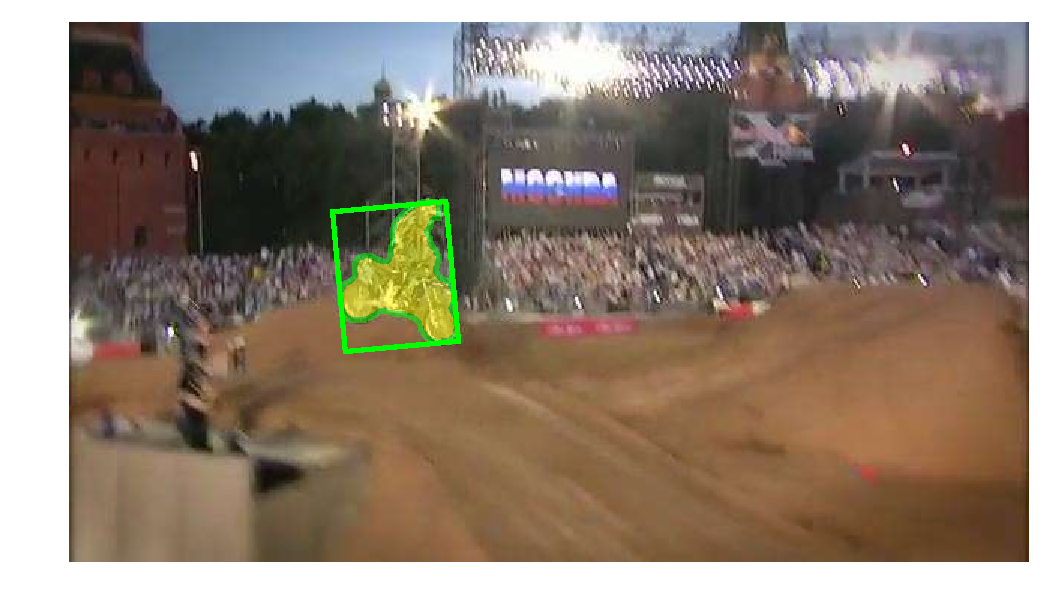
\includegraphics[trim={2.5cm 1cm 2.5cm 1cm},clip,width = 1.1in]{supp/vot2018/pdf/motocross1/00035}
& 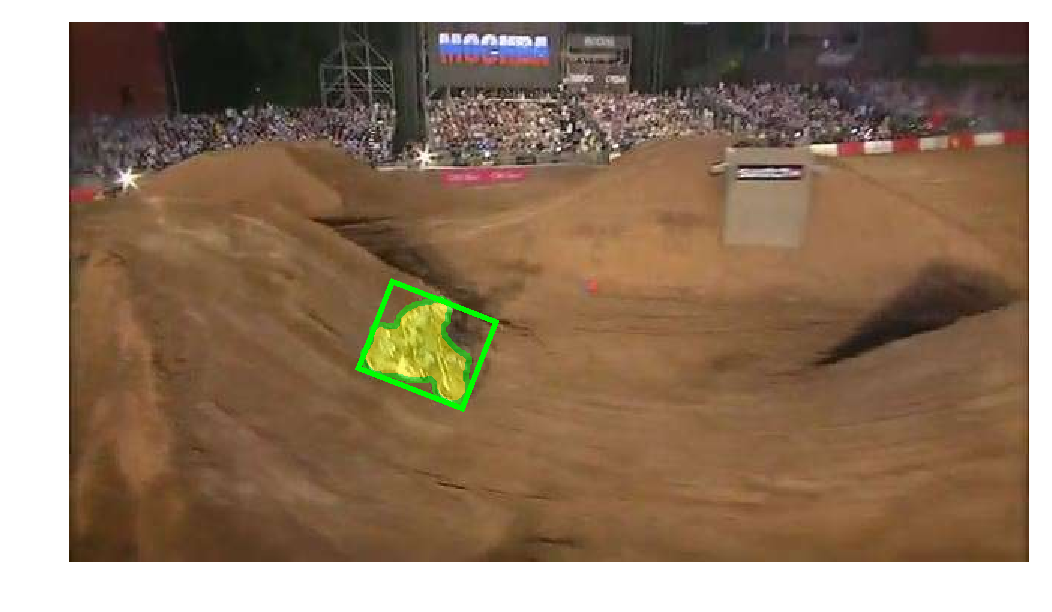
\includegraphics[trim={2.5cm 1cm 2.5cm 1cm},clip,width = 1.1in]{supp/vot2018/pdf/motocross1/00050}
& 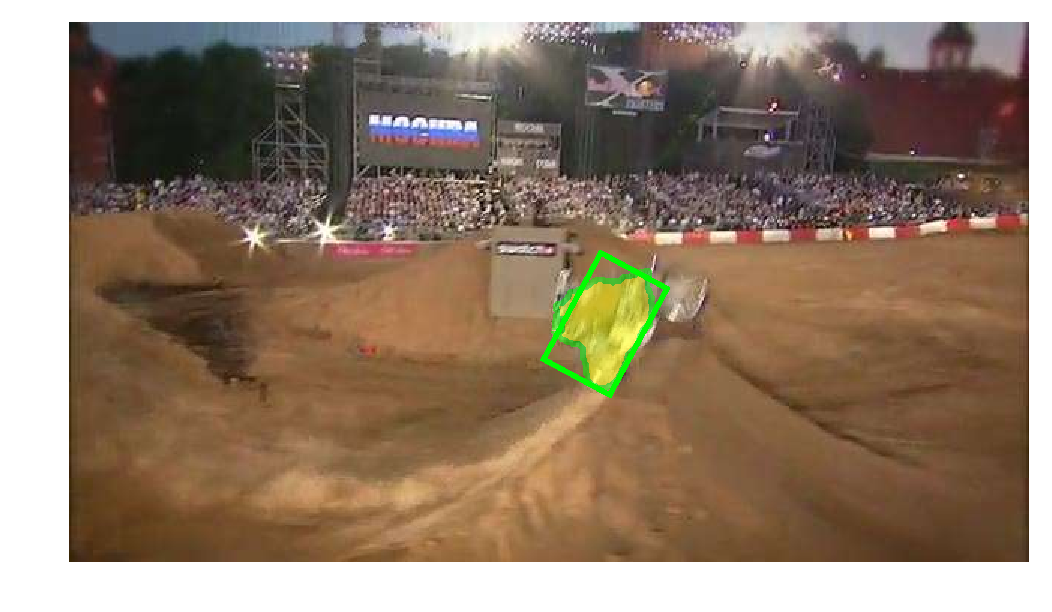
\includegraphics[trim={2.5cm 1cm 2.5cm 1cm},clip,width = 1.1in]{supp/vot2018/pdf/motocross1/00069}
& 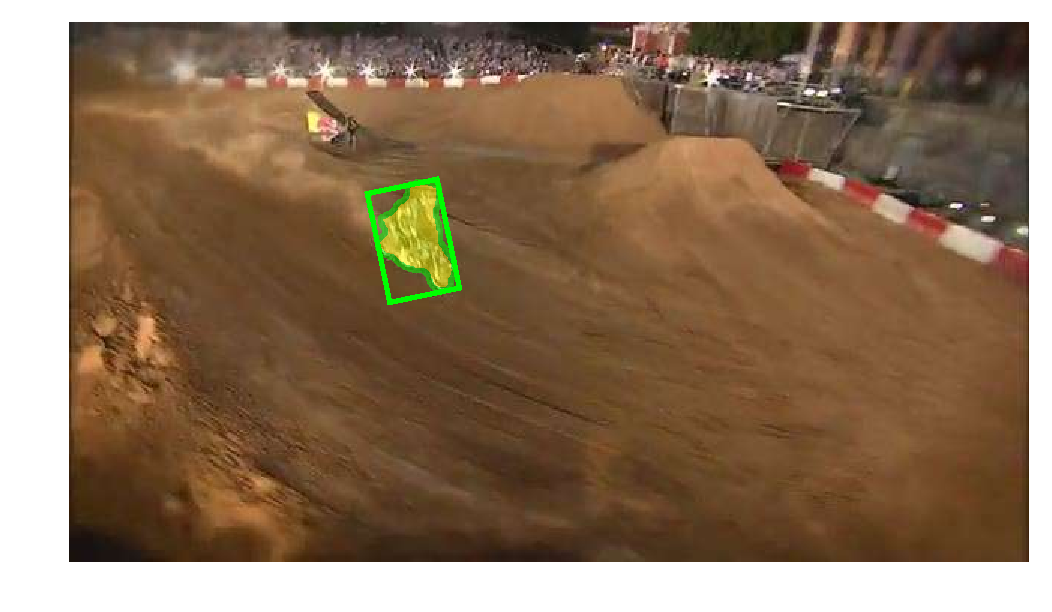
\includegraphics[trim={2.5cm 1cm 2.5cm 1cm},clip,width = 1.1in]{supp/vot2018/pdf/motocross1/00140}
\\
\mbox{\rotatebox[x=-0.2cm]{90}{\small{singer2}}}
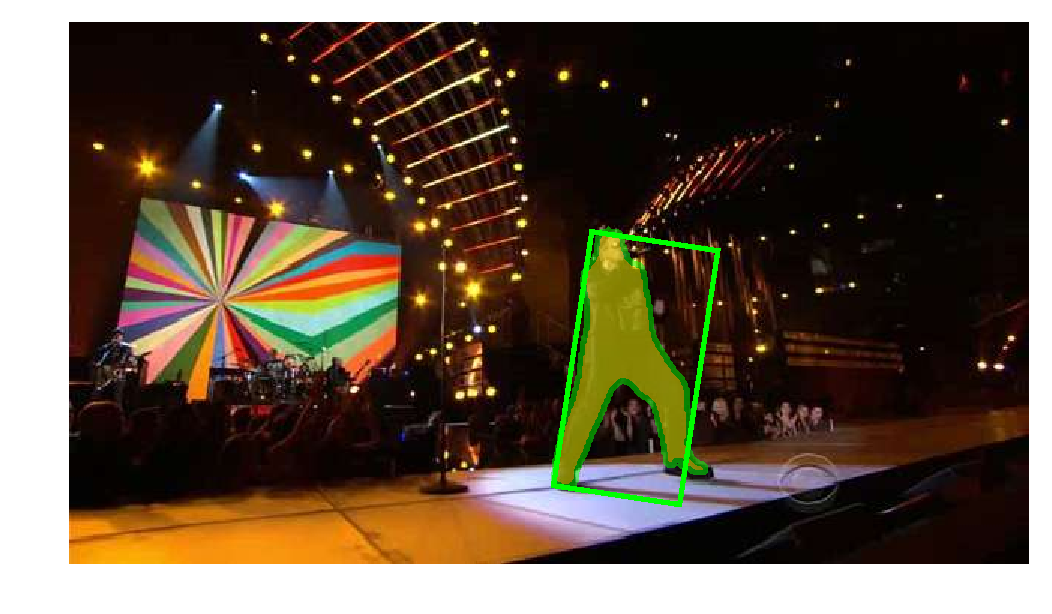
\includegraphics[trim={2.5cm 1cm 2.5cm 1cm},clip,width = 1.1in]{supp/vot2018/pdf/singer2/00057}
&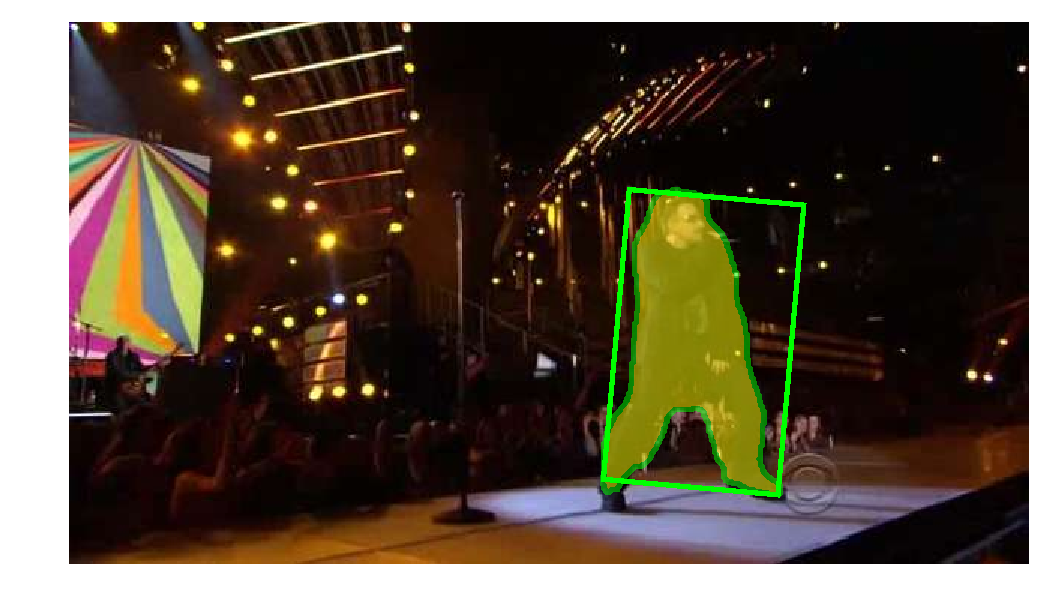
\includegraphics[trim={2.5cm 1cm 2.5cm 1cm},clip,width = 1.1in]{supp/vot2018/pdf/singer2/00141}
& 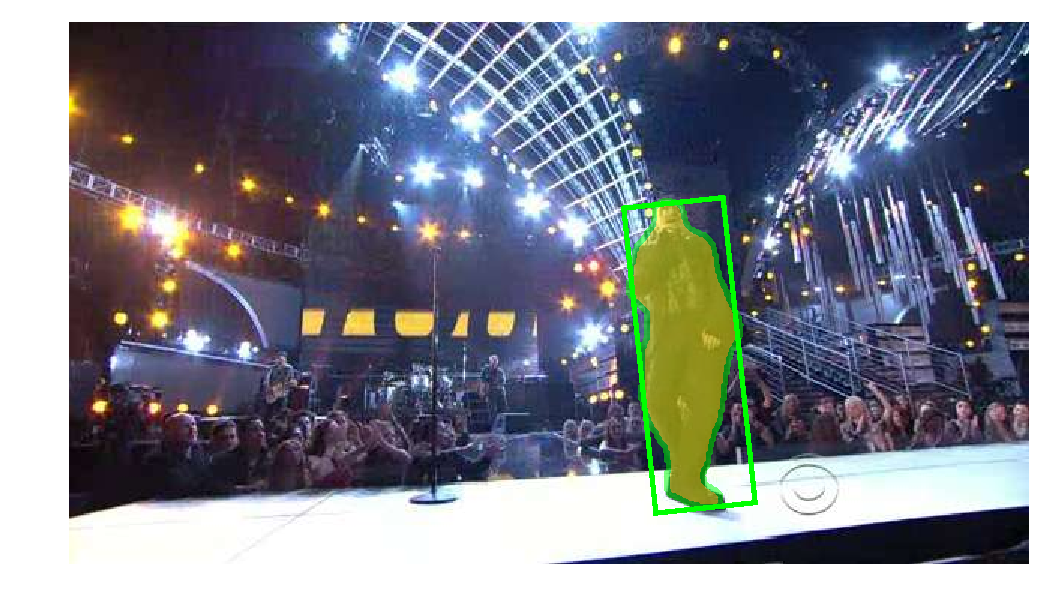
\includegraphics[trim={2.5cm 1cm 2.5cm 1cm},clip,width = 1.1in]{supp/vot2018/pdf/singer2/00232}
& 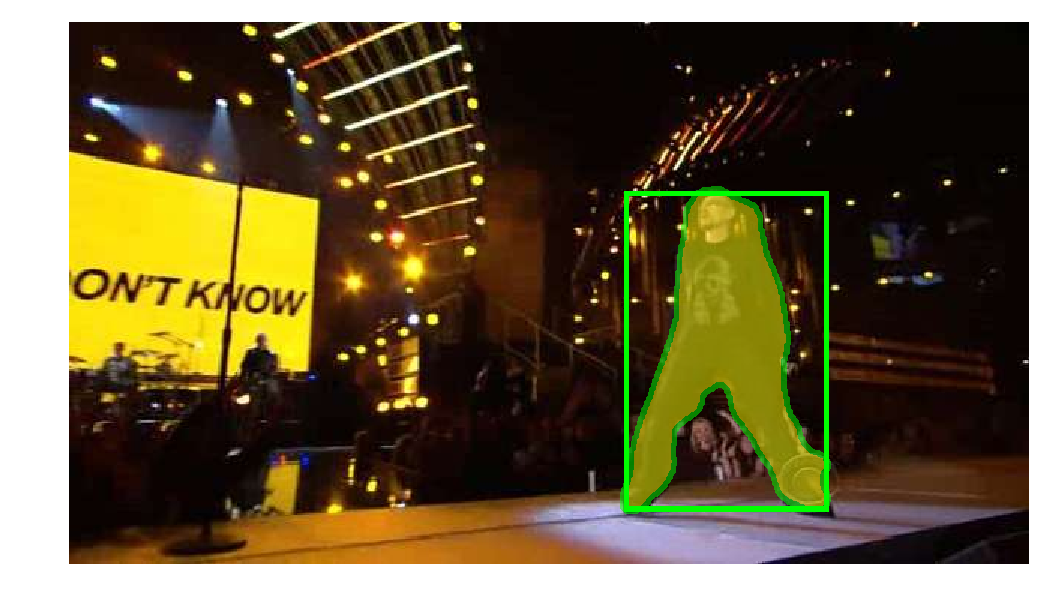
\includegraphics[trim={2.5cm 1cm 2.5cm 1cm},clip,width = 1.1in]{supp/vot2018/pdf/singer2/00283}
& 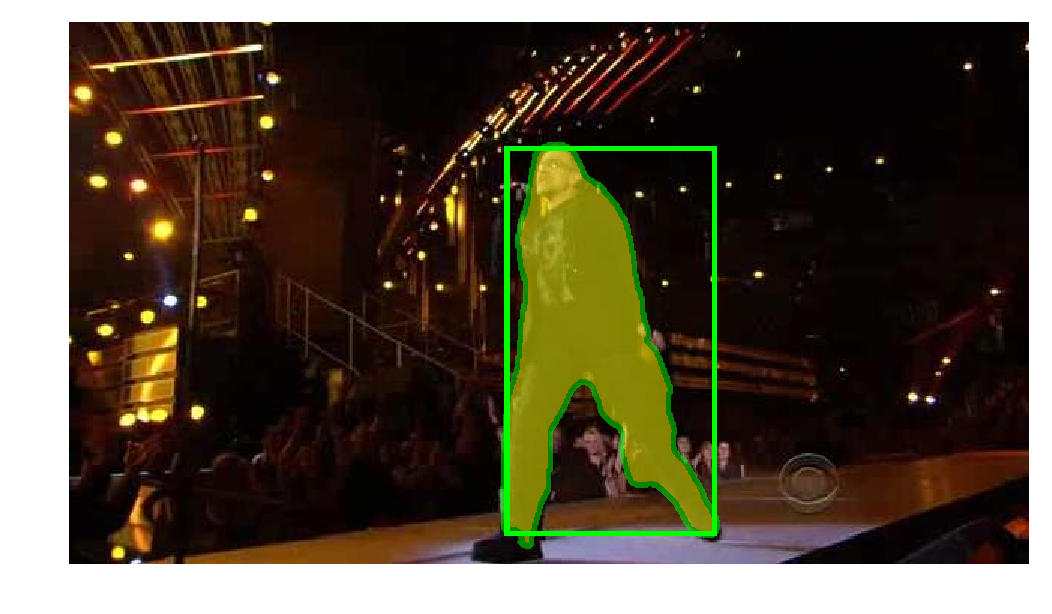
\includegraphics[trim={2.5cm 1cm 2.5cm 1cm},clip,width = 1.1in]{supp/vot2018/pdf/singer2/00335}
& 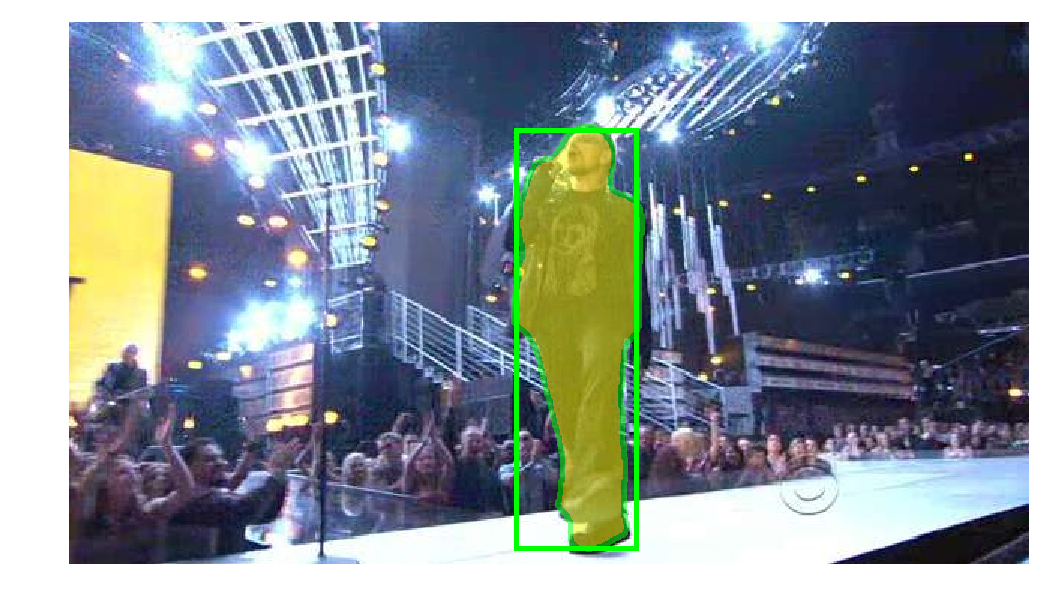
\includegraphics[trim={2.5cm 1cm 2.5cm 1cm},clip,width = 1.1in]{supp/vot2018/pdf/singer2/00348}
\\
\mbox{\rotatebox[x=-0.55cm]{90}{\small{soccer1}}}
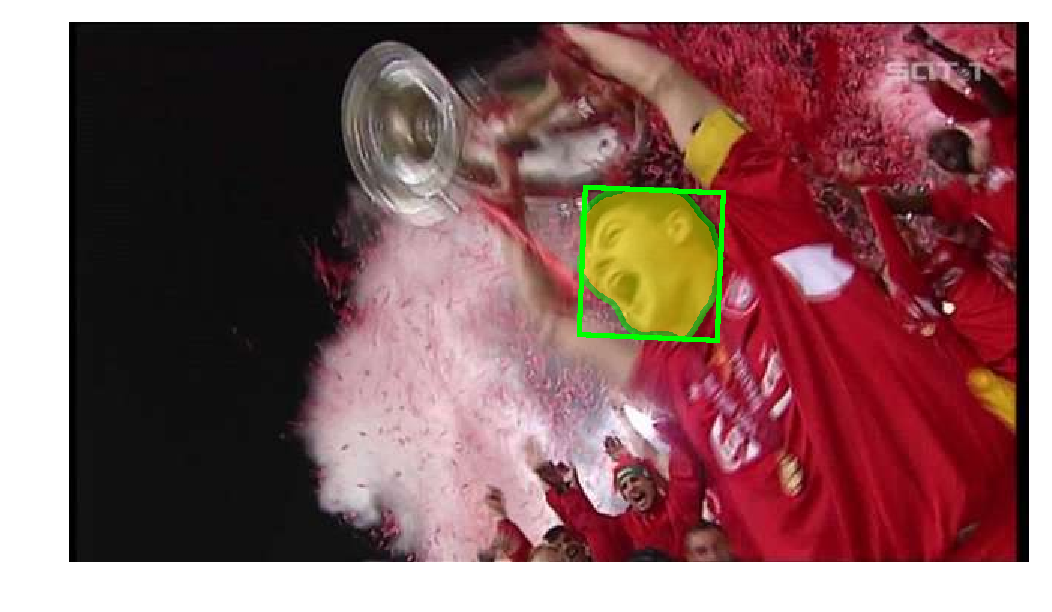
\includegraphics[trim={2.5cm 1cm 2.5cm 1cm},clip,width = 1.1in]{supp/vot2018/pdf/soccer1/00021}
&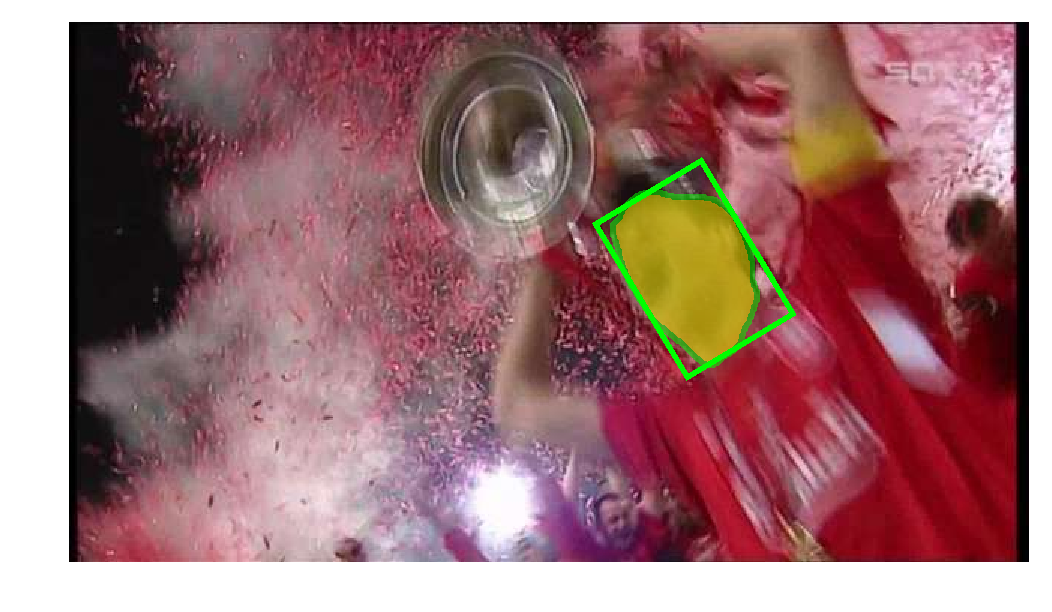
\includegraphics[trim={2.5cm 1cm 2.5cm 1cm},clip,width = 1.1in]{supp/vot2018/pdf/soccer1/00039}
& 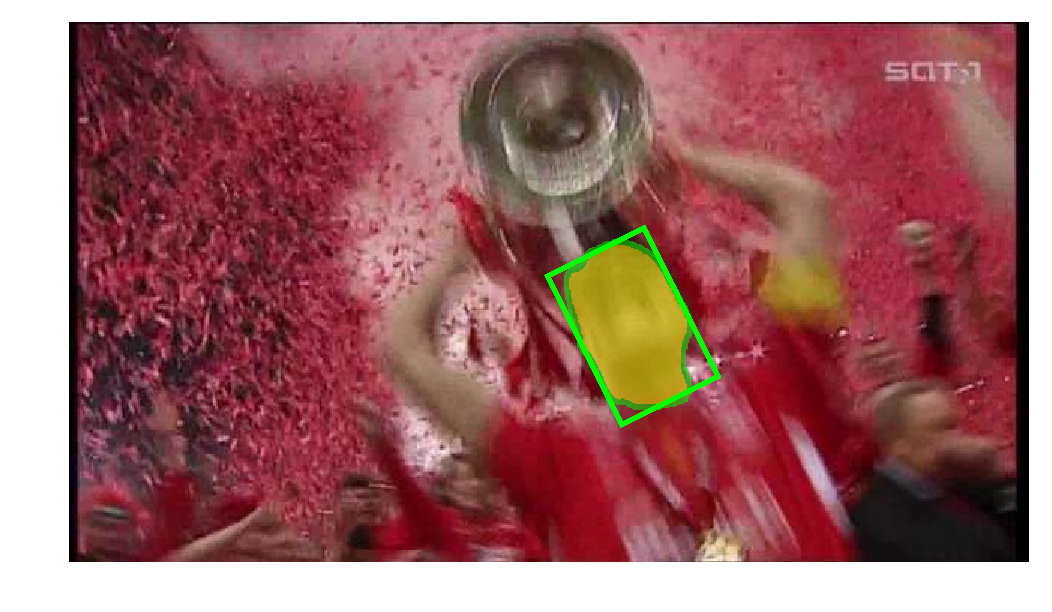
\includegraphics[trim={2.5cm 1cm 2.5cm 1cm},clip,width = 1.1in]{supp/vot2018/pdf/soccer1/00061}
& 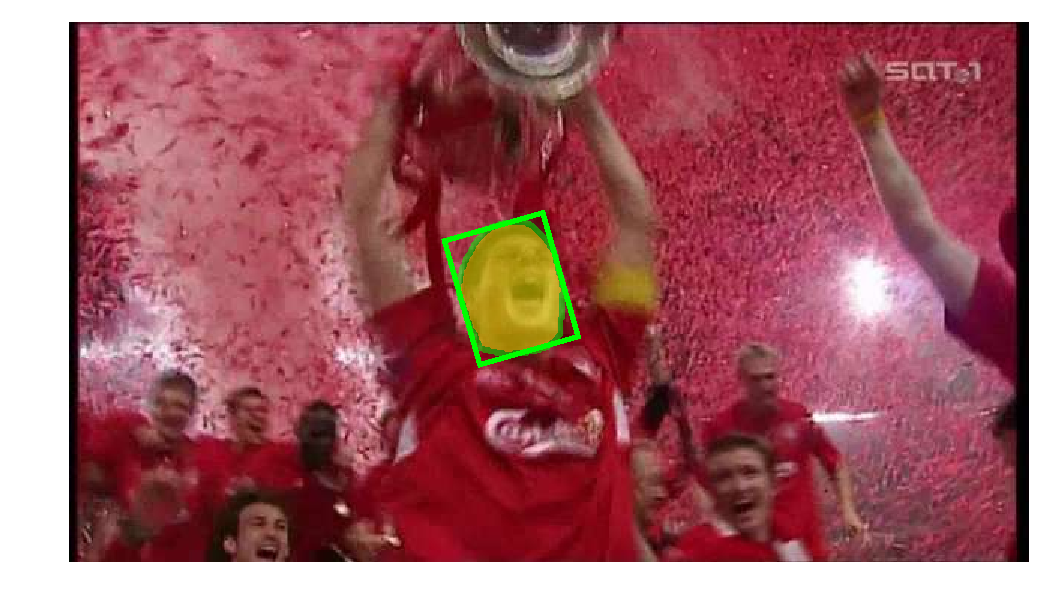
\includegraphics[trim={2.5cm 1cm 2.5cm 1cm},clip,width = 1.1in]{supp/vot2018/pdf/soccer1/00079}
& 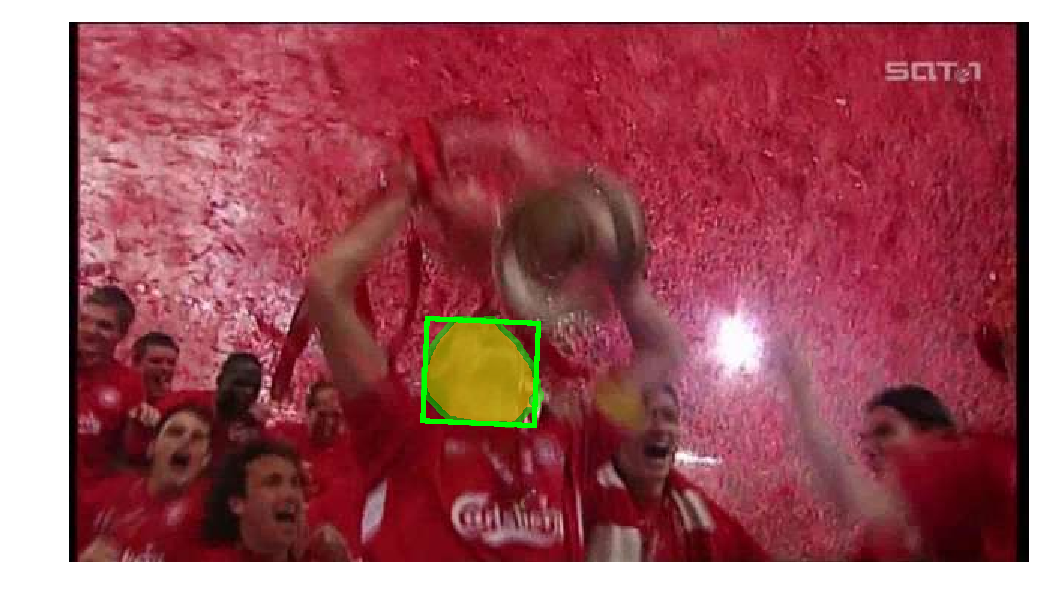
\includegraphics[trim={2.5cm 1cm 2.5cm 1cm},clip,width = 1.1in]{supp/vot2018/pdf/soccer1/00090}
& 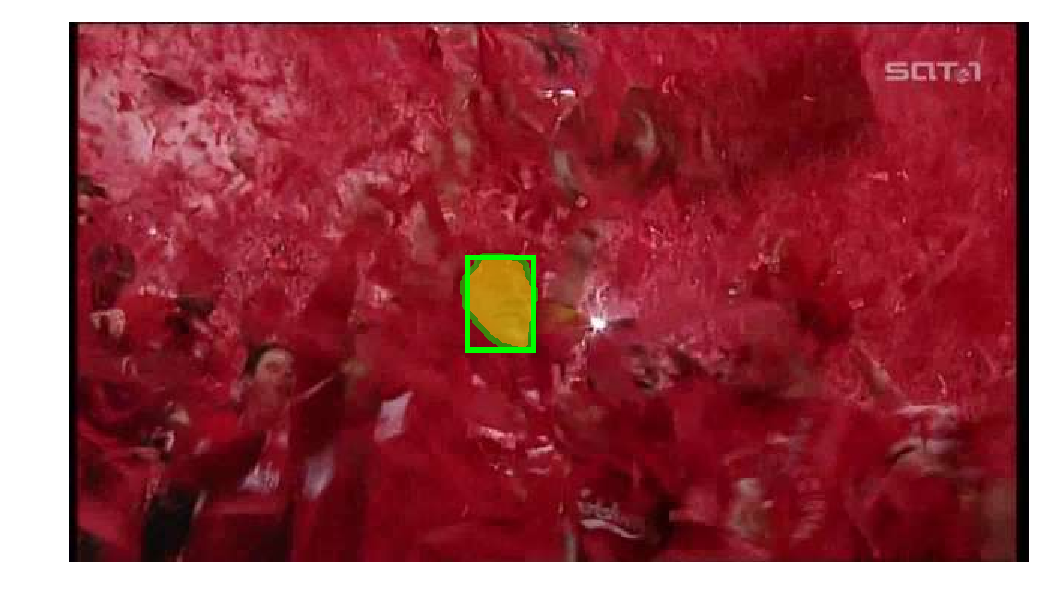
\includegraphics[trim={2.5cm 1cm 2.5cm 1cm},clip,width = 1.1in]{supp/vot2018/pdf/soccer1/00110}
\\
\end{tabular}

\vspace{-0.2cm}
\caption{Further qualitative results of our method on sequences from the visual object tracking benchmark VOT-2018~\cite{VOT2018}.}
\label{fig:appendix_vot18}
\end{figure*}


\begin{figure*}
\centering
\setlength{\tabcolsep}{0.25ex}

\begin{tabular}
{cccccc cccccc}




\mbox{\rotatebox[x=-0.55cm]{90}{\small{dog}}}
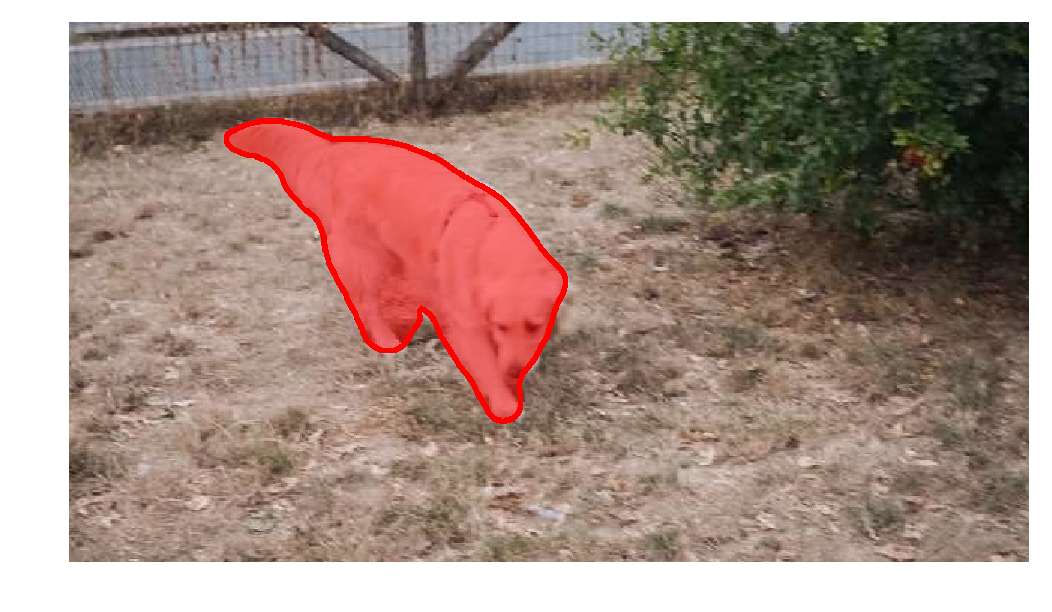
\includegraphics[trim={2.5cm 1cm 2.5cm 1cm},clip,width = 1.1in]{supp/davis16/pdf/dog/00007}
&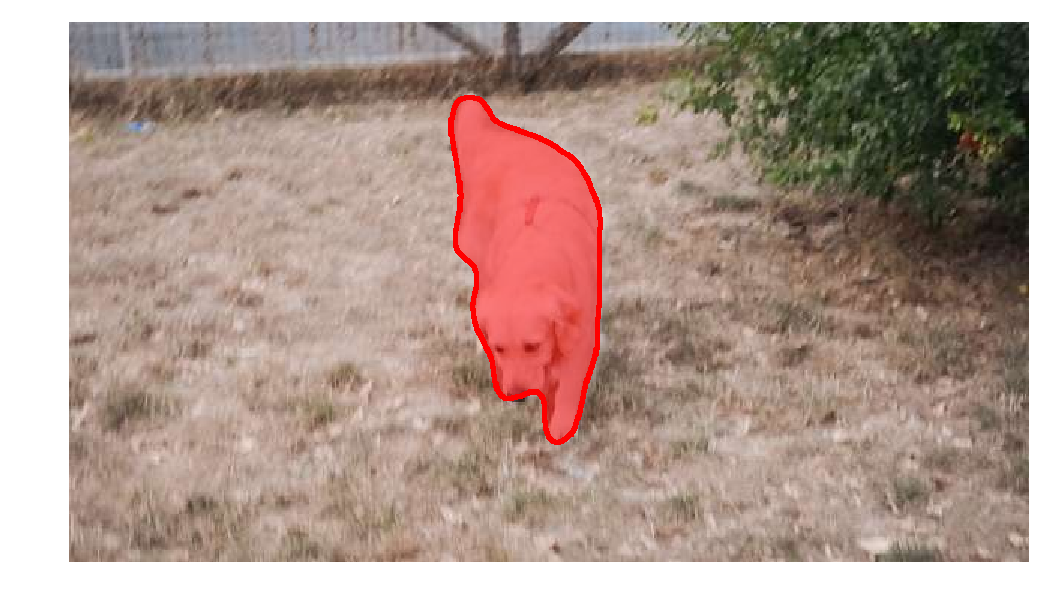
\includegraphics[trim={2.5cm 1cm 2.5cm 1cm},clip,width = 1.1in]{supp/davis16/pdf/dog/00020}
& 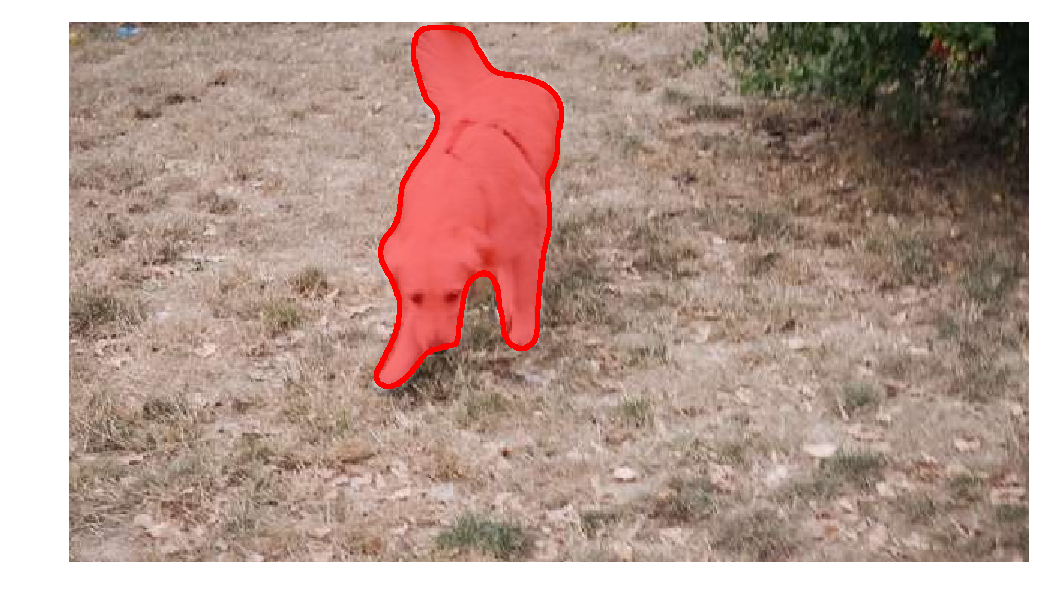
\includegraphics[trim={2.5cm 1cm 2.5cm 1cm},clip,width = 1.1in]{supp/davis16/pdf/dog/00028}
& 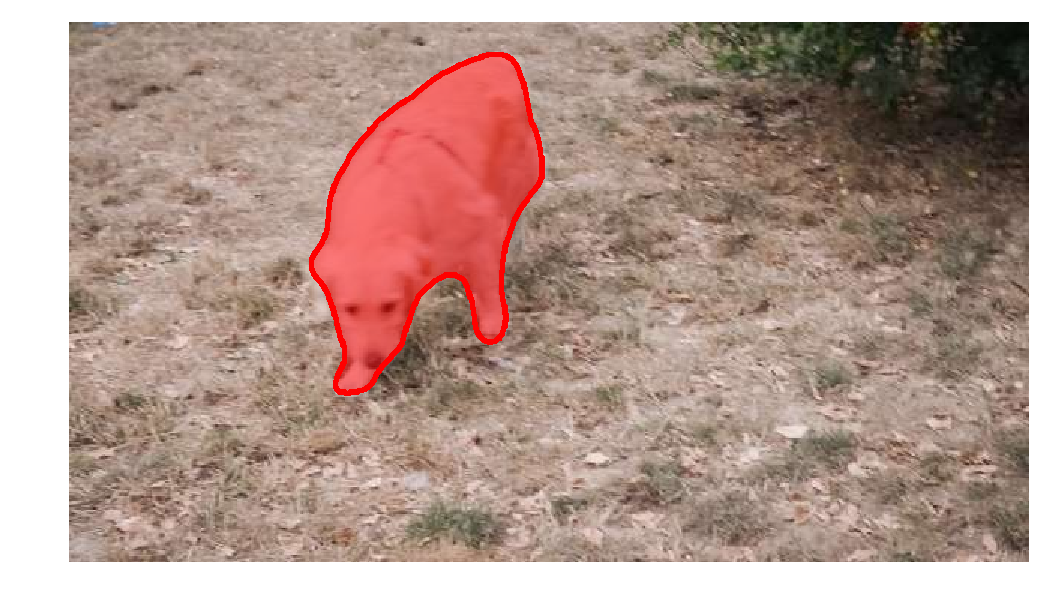
\includegraphics[trim={2.5cm 1cm 2.5cm 1cm},clip,width = 1.1in]{supp/davis16/pdf/dog/00032}
& 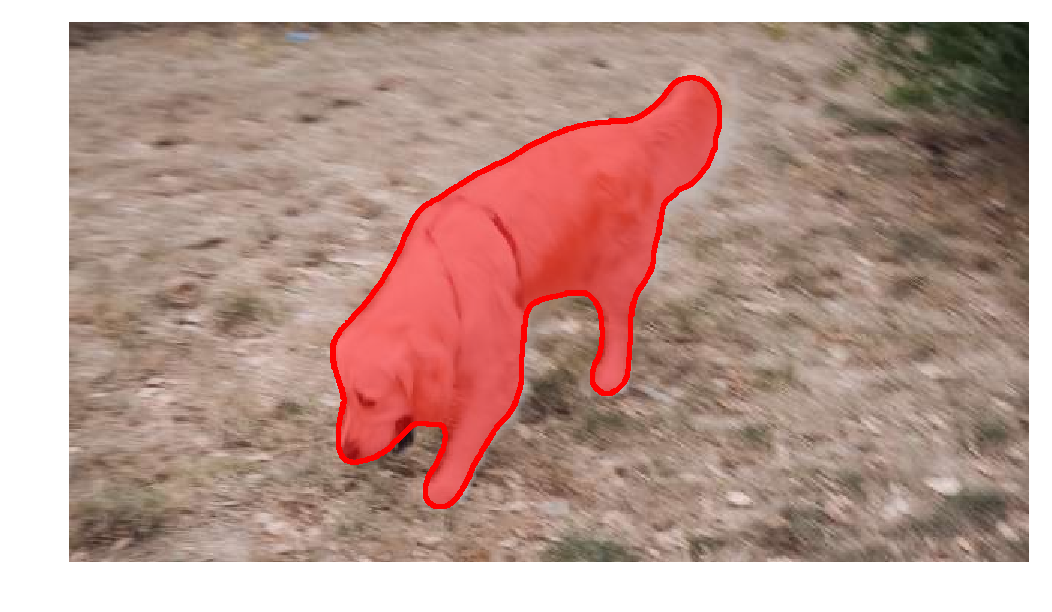
\includegraphics[trim={2.5cm 1cm 2.5cm 1cm},clip,width = 1.1in]{supp/davis16/pdf/dog/00044}
& \includegraphics[trim={2.5cm 1cm 2.5cm 1cm},clip,width = 1.1in]{supp/davis16/pdf/dog/00050}
\\

\mbox{\rotatebox[x=-0.cm]{90}{\small{drift-straight}}}
\includegraphics[trim={2.5cm 1cm 2.5cm 1cm},clip,width = 1.1in]{supp/davis16/pdf/drift-straight/00003}
&\includegraphics[trim={2.5cm 1cm 2.5cm 1cm},clip,width = 1.1in]{supp/davis16/pdf/drift-straight/00017}
& \includegraphics[trim={2.5cm 1cm 2.5cm 1cm},clip,width = 1.1in]{supp/davis16/pdf/drift-straight/00027}
& \includegraphics[trim={2.5cm 1cm 2.5cm 1cm},clip,width = 1.1in]{supp/davis16/pdf/drift-straight/00031}
& \includegraphics[trim={2.5cm 1cm 2.5cm 1cm},clip,width = 1.1in]{supp/davis16/pdf/drift-straight/00036}
& \includegraphics[trim={2.5cm 1cm 2.5cm 1cm},clip,width = 1.1in]{supp/davis16/pdf/drift-straight/00047}
\\

\mbox{\rotatebox[x=-0.55cm]{90}{\small{goat}}}
\includegraphics[trim={2.5cm 1cm 2.5cm 1cm},clip,width = 1.1in]{supp/davis16/pdf/goat/00000}
&\includegraphics[trim={2.5cm 1cm 2.5cm 1cm},clip,width = 1.1in]{supp/davis16/pdf/goat/00014}
& \includegraphics[trim={2.5cm 1cm 2.5cm 1cm},clip,width = 1.1in]{supp/davis16/pdf/goat/00025}
& \includegraphics[trim={2.5cm 1cm 2.5cm 1cm},clip,width = 1.1in]{supp/davis16/pdf/goat/00036}
& \includegraphics[trim={2.5cm 1cm 2.5cm 1cm},clip,width = 1.1in]{supp/davis16/pdf/goat/00045}
& \includegraphics[trim={2.5cm 1cm 2.5cm 1cm},clip,width = 1.1in]{supp/davis16/pdf/goat/00067}
\\


\mbox{\rotatebox[x=-0.55cm]{90}{\small{Libby}}}
\includegraphics[trim={2.5cm 1cm 2.5cm 1cm},clip,width = 1.1in]{supp/davis16/pdf/libby/00000}
&\includegraphics[trim={2.5cm 1cm 2.5cm 1cm},clip,width = 1.1in]{supp/davis16/pdf/libby/00016}
& \includegraphics[trim={2.5cm 1cm 2.5cm 1cm},clip,width = 1.1in]{supp/davis16/pdf/libby/00035}
& \includegraphics[trim={2.5cm 1cm 2.5cm 1cm},clip,width = 1.1in]{supp/davis16/pdf/libby/00039}
& \includegraphics[trim={2.5cm 1cm 2.5cm 1cm},clip,width = 1.1in]{supp/davis16/pdf/libby/00045}
& \includegraphics[trim={2.5cm 1cm 2.5cm 1cm},clip,width = 1.1in]{supp/davis16/pdf/libby/00048}
\\

\mbox{\rotatebox[x=-0.cm]{90}{\scriptsize{motocross-jump}}}
\includegraphics[trim={2.5cm 1cm 2.5cm 1cm},clip,width = 1.1in]{supp/davis16/pdf/motocross-jump/00004}
&\includegraphics[trim={2.5cm 1cm 2.5cm 1cm},clip,width = 1.1in]{supp/davis16/pdf/motocross-jump/00010}
& \includegraphics[trim={2.5cm 1cm 2.5cm 1cm},clip,width = 1.1in]{supp/davis16/pdf/motocross-jump/00027}
& \includegraphics[trim={2.5cm 1cm 2.5cm 1cm},clip,width = 1.1in]{supp/davis16/pdf/motocross-jump/00033}
& \includegraphics[trim={2.5cm 1cm 2.5cm 1cm},clip,width = 1.1in]{supp/davis16/pdf/motocross-jump/00037}
& \includegraphics[trim={2.5cm 1cm 2.5cm 1cm},clip,width = 1.1in]{supp/davis16/pdf/motocross-jump/00039}
\\


\mbox{\rotatebox[x=-0.55cm]{90}{\small{parkour}}}
\includegraphics[trim={2.5cm 1cm 2.5cm 0.5cm},clip,width = 1.1in]{supp/davis16/pdf/parkour/00000}
&\includegraphics[trim={2.5cm 1cm 2.5cm 0.5cm},clip,width = 1.1in]{supp/davis16/pdf/parkour/00016}
& \includegraphics[trim={2.5cm 1cm 2.5cm 0.5cm},clip,width = 1.1in]{supp/davis16/pdf/parkour/00033}
& \includegraphics[trim={2.5cm 1cm 2.5cm 0.5cm},clip,width = 1.1in]{supp/davis16/pdf/parkour/00043}
& \includegraphics[trim={2.5cm 1cm 2.5cm 0.5cm},clip,width = 1.1in]{supp/davis16/pdf/parkour/00047}
& \includegraphics[trim={2.5cm 1cm 2.5cm 0.5cm},clip,width = 1.1in]{supp/davis16/pdf/parkour/00090}
\\
\mbox{\rotatebox[x=-0.0cm]{90}{\small{Gold-Fish}}}
\includegraphics[trim={2.5cm 1cm 2.5cm 1cm},clip,width = 1.1in]{img/davis16/pdf/gold-fish/00003}
&\includegraphics[trim={2.5cm 1cm 2.5cm 1cm},clip,width = 1.1in]{img/davis16/pdf/gold-fish/00012}
& \includegraphics[trim={2.5cm 1cm 2.5cm 1cm},clip,width = 1.1in]{img/davis16/pdf/gold-fish/00020}
& \includegraphics[trim={2.5cm 1cm 2.5cm 1cm},clip,width = 1.1in]{img/davis16/pdf/gold-fish/00054}
& \includegraphics[trim={2.5cm 1cm 2.5cm 1cm},clip,width = 1.1in]{img/davis16/pdf/gold-fish/00060}
& \includegraphics[trim={2.5cm 1cm 2.5cm 1cm},clip,width = 1.1in]{img/davis16/pdf/gold-fish/00070}
\\


\end{tabular}

\caption{Further qualitative results of our method on sequences from the semi-supervised video object segmentation benchmarks DAVIS-2016~\cite{perazzi2016benchmark} and DAVIS-2017~\cite{pont2017davis}.
Multiple masks are obtained from different inferences (with different initialisations).
}
\label{fig:appendix_davis16}
\end{figure*}
